\documentclass[11pt]{article}

% Change "review" to "final" to generate the final (sometimes called camera-ready) version.
% Change to "preprint" to generate a non-anonymous version with page numbers.
% \usepackage[review]{acl}
\usepackage[preprint]{acl}
% Standard package includes
\usepackage{times}
\usepackage{latexsym}

% For proper rendering and hyphenation of words containing Latin characters (including in bib files)
\usepackage[T1]{fontenc}
% For Vietnamese characters
% \usepackage[T5]{fontenc}
% See https://www.latex-project.org/help/documentation/encguide.pdf for other character sets

% This assumes your files are encoded as UTF8
\usepackage[utf8]{inputenc}
\usepackage{amssymb}

% This is not strictly necessary, and may be commented out,
% but it will improve the layout of the manuscript,
% and will typically save some space.
\usepackage{microtype}

\usepackage{inconsolata}
\usepackage{graphicx}
\usepackage{kotex}

\usepackage{booktabs}
\usepackage{multirow}
\usepackage{enumitem}
\usepackage{array}
\usepackage{listings}
\usepackage{amsmath} 
\usepackage{tcolorbox}
\tcbuselibrary{skins}
\usepackage{tabularx}
\usepackage{capt-of}
\usepackage{placeins}
% \usepackage[most]{tcolorbox}
% \tcbuselibrary{skins,breakable}


\newcommand{\eg}{\emph{e.g.}}
\newcommand{\Eg}{\emph{E.g.}}
\newcommand{\ie}{\emph{i.e.}}
\newcommand{\Ie}{\emph{I.e.}}
\newcommand{\cf}{\emph{cf.}}
\newcommand{\Cf}{\emph{Cf.}}
\newcommand{\etc}{\emph{etc.}}
\newcommand{\vs}{\emph{vs.}}
\newcommand{\wrt}{w.r.t.}
\newcommand{\dof}{d.o.f.}
\newcommand{\iid}{i.i.d.}
\newcommand{\wolog}{w.l.o.g.}

\newcommand{\figref}[1]{Figure~\ref{#1}}
\newcommand{\tabref}[1]{Table~\ref{#1}}
\newcommand{\equref}[1]{Eq.~(\ref{#1})}
\newcommand{\algref}[1]{Alg.~(\ref{#1})}
\newcommand{\secref}[1]{Section~\ref{#1}}

\lstset{
  basicstyle=\ttfamily\small,
  breaklines=true,
  columns=fullflexible,
  frame=single,
  showstringspaces=false
}
\usepackage[table]{xcolor}
\usepackage{colortbl}
\usepackage{pifont} % <-- \ding 사용에 필요
\usepackage{siunitx}
\usepackage{arydshln}

\sisetup{
  round-mode      = places,
  round-precision = 1,
  round-half      = up,
  detect-all      = true
}

\definecolor{Green}{RGB}{30,130,30}
% \newcommand{\cmark}{\textcolor{Green}{\ding{51}}} 
% \newcommand{\xmark}{\textcolor{red}{\ding{55}}}   
\newcommand{\cmark}{\ding{51}} 
\newcommand{\xmark}{\ding{55}}   
% If the title and author information does not fit in the area allocated, uncomment the following
%
%\setlength\titlebox{<dim>}
%
% and set <dim> to something 5cm or larger.

\title{TCVP: A Practical Pipeline for Video Moment Retrieval Datasets \\Leveraging Timestamped Video Comments}

\input{input/author}

\begin{document}
\maketitle
\begin{abstract} 
Video Moment Retrieval (VMR) aims to identify a temporal moment in a video that corresponds to a user query.
Most existing VMR datasets are constructed by randomly selecting temporal moments and generating queries from the corresponding visual and auditory content. 
We find that this process often produces moments with limited importance and queries that resemble captions rather than user-driven searches.
To address these limitations, we propose a practical pipeline for VMR dataset generation, named TCVP, where we leverage timestamped YouTube comments to identify interesting moments and reflect actual search intent.
A naive use of YouTube comments introduces several challenges, as many comments are uninformative (\eg, “07:22 lol”), and comments may correspond to different modalities, requiring modality-aware handling.
Our pipeline alleviates them by introducing comment filtering and modality gating as key methodological components.
Our qualitative analysis shows that users prefer our dataset by a substantial margin (\ie, 70\%) over existing baselines. 
Moreover, benchmarking models on our dataset highlights limitations of current VMR methods and offers insights for future work.
Our dataset and code are publicly available at \url{https://jung0228.github.io/TCVP/}. 
\end{abstract}

% pdf로 바꾸어서 넣기. 
\begin{figure*}[t]
  \centering
  \resizebox{\linewidth}{!}{
    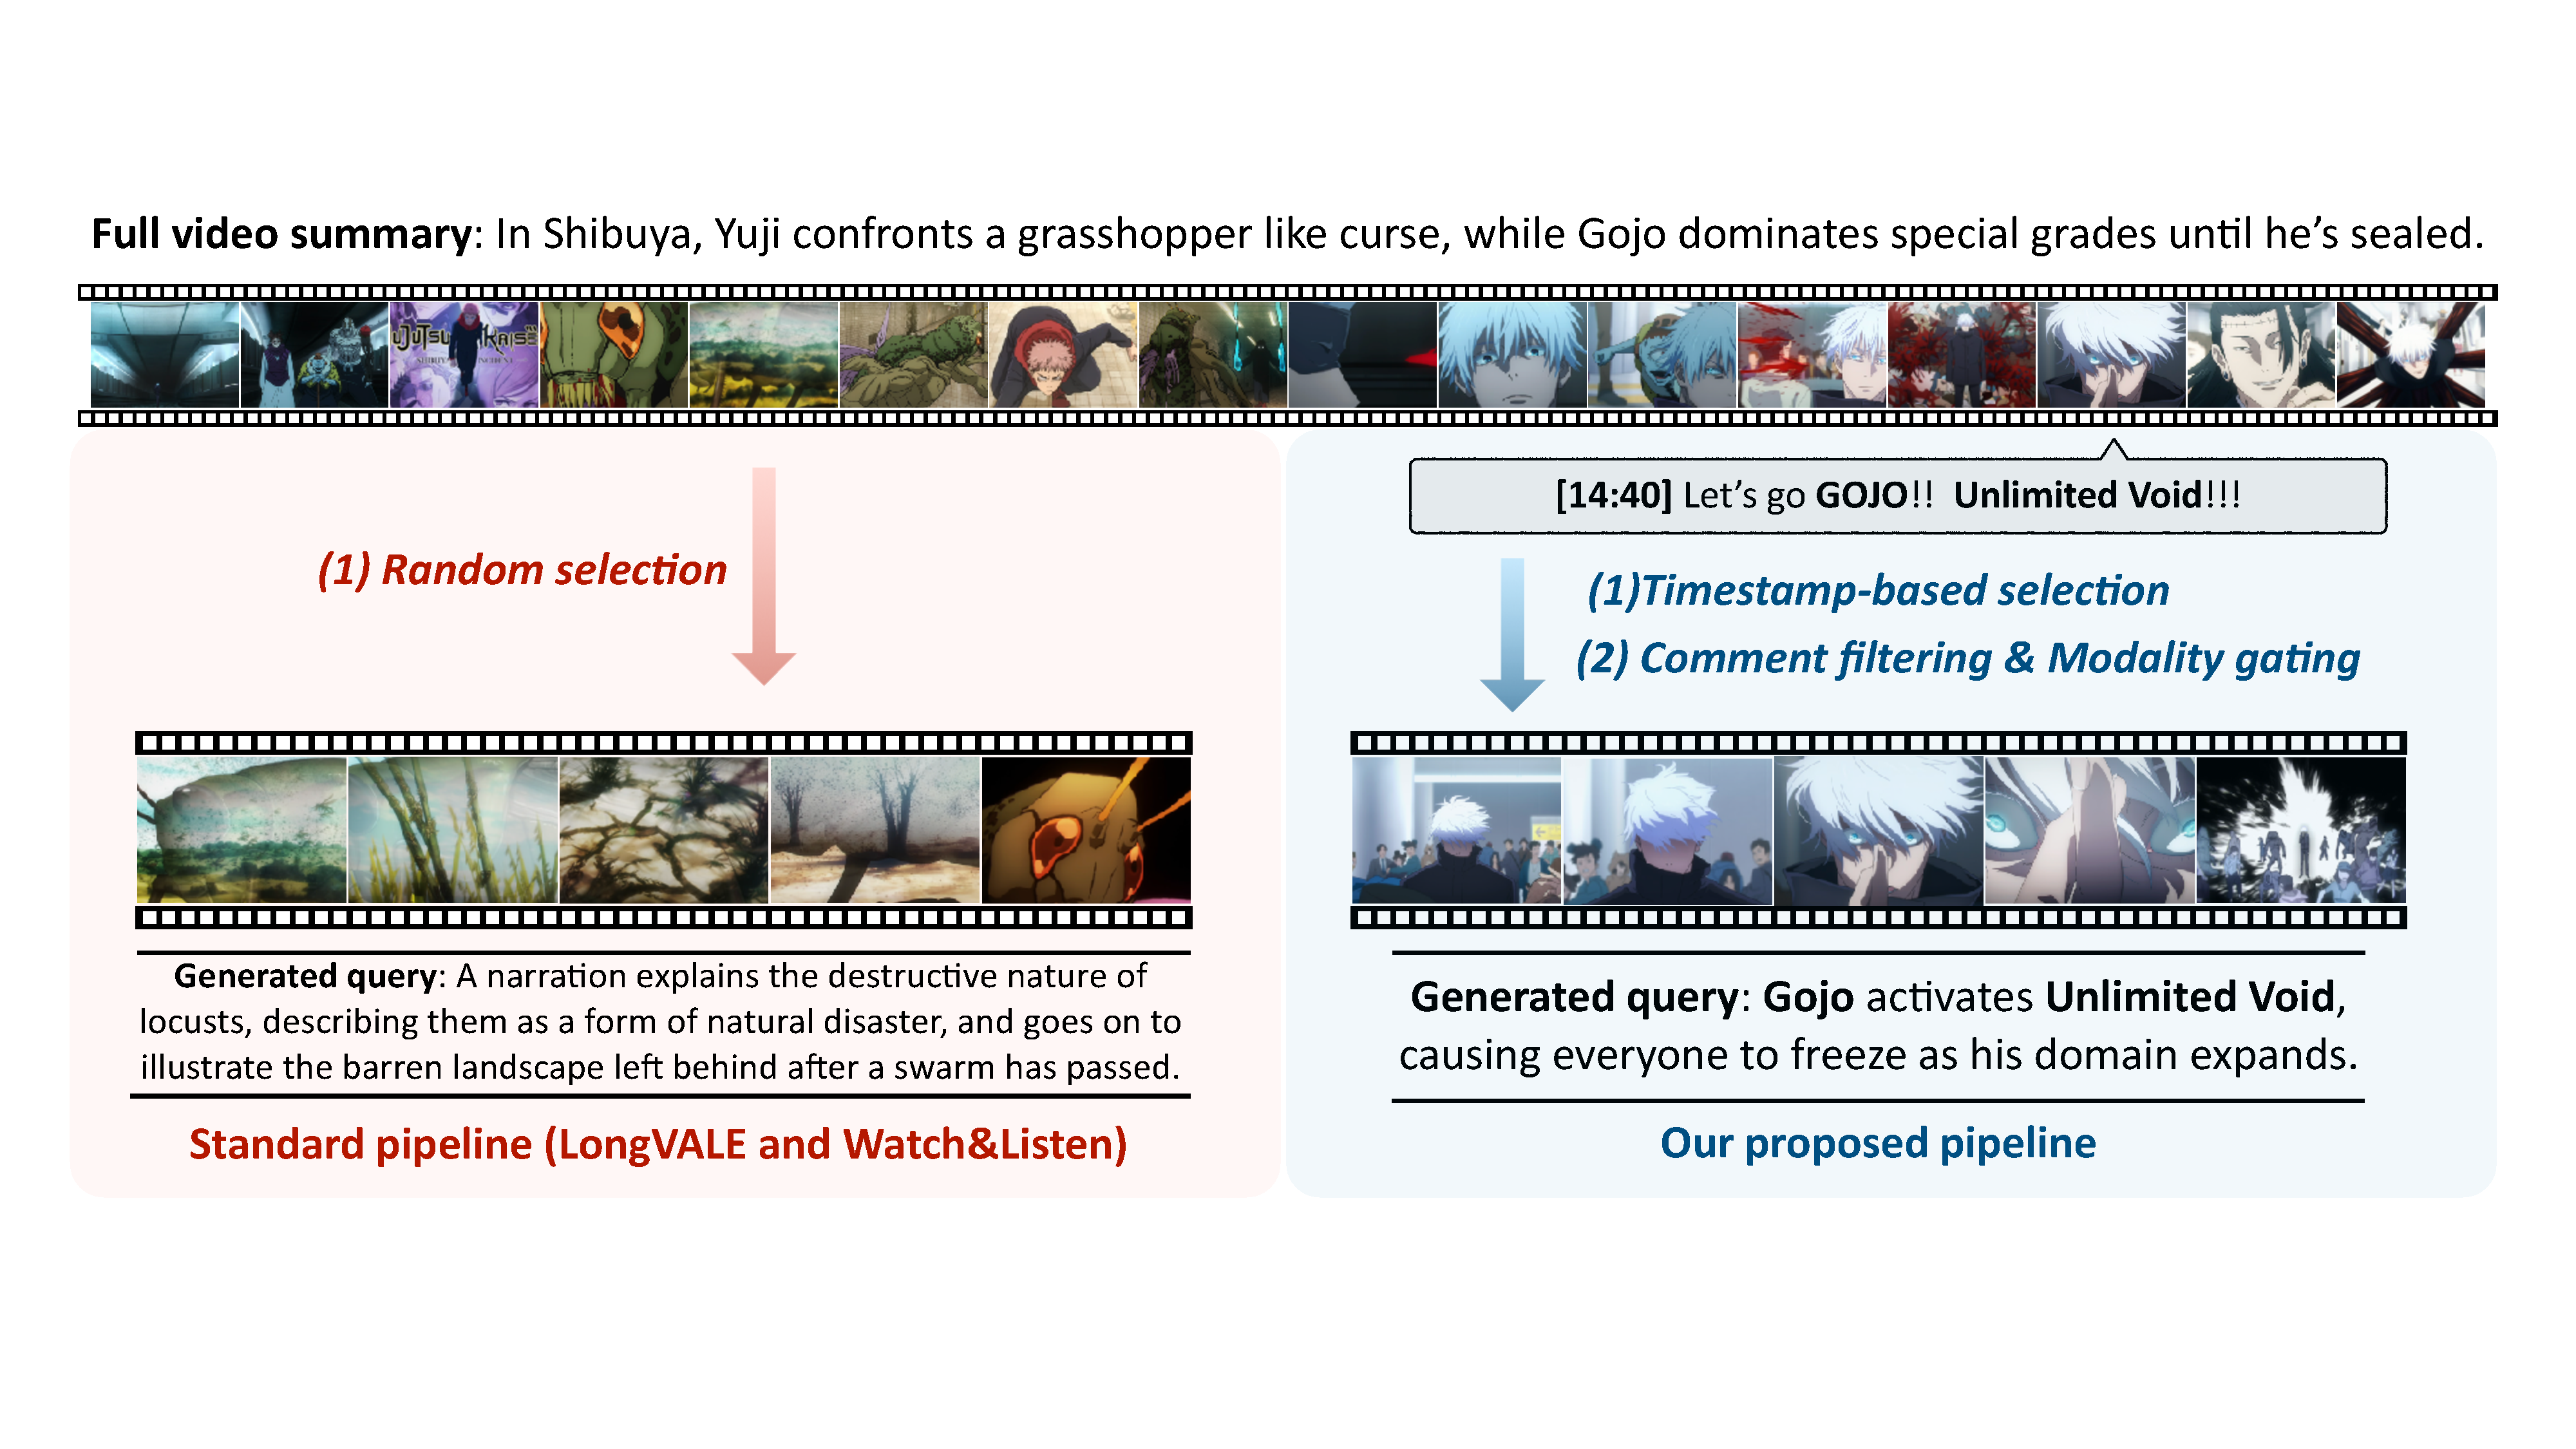
\includegraphics[width=\textwidth]{image/pipeline_comparison.pdf}
  }
  \vspace{-1.8em}
  \caption{Comparison between our comment based pipeline and a standard pipeline. Our method selects moments using timestamped user comments with modality-aware filtering to generate natural, whereas standard pipelines selects effectively random moments.}
  \label{fig:pipeline}
\vspace{-1.em}
\end{figure*}
\vspace{+1em}
\section{Introduction}
Given a natural language query, the goal of Video Moment Retrieval (VMR) is to locate the corresponding temporal moments within a video~\cite{lei2021detecting, moon2023query, ren2024timechat, pan2025timesearch}.
This capability is useful in diverse scenarios, such as assisting video editors in identifying salient moments from lengthy recordings~\cite{huh2025videodiff, croitoru2023moment}, or enabling Netflix users to search for specific scenes they wish to revisit in previously watched videos~\cite{chen2023invideosearch}.
By reducing the need for manual exploration, VMR can serve as a practical tool in user-facing applications.

% To enable the development and evaluation of VMR models, existing studies~\cite{gao2017tall,lei2020tvr,lei2021detecting,lin2023univtg, soldan2022mad} have introduced VMR datasets.
To enable the development and evaluation of VMR models, existing studies have introduced VMR datasets~\cite{gao2017tall,lei2020tvr,lei2021detecting,lin2023univtg, soldan2022mad}. 

\figref{fig:pipeline} (red boxes) illustrates a representative data generation pipeline used in these works.
As shown, this pipeline often yields moments that are weakly aligned with real user interest and queries that are verbose and descriptive rather than search-oriented. 
We \textit{identify} this mismatch as a fundamental limitation of existing VMR datasets, motivating the need for datasets that better reflect real user intent.

To address this gap, we present a new perspective by leveraging timestamped YouTube comments.
These comments naturally indicate which moments users consider important and how they refer to them in practice. 
Based on this observation, we propose a simple-yet-effective dataset construction pipeline, termed the \textbf{T}imestamped \textbf{C}omment-guided \textbf{V}MR \textbf{P}ipeline (\textbf{TCVP}).
Directly using the comments poses challenges, as many are uninformative and user reactions may focus on different modalities, which necessitates modality-specific data construction procedures. For example, some comments express general reactions or emotions, while others target specific either visual events or audio content. Hence, TCVP incorporates comment filtering and modality gating.
Comment filtering removes irrelevant or weakly grounded comments, while modality gating assigns the remaining ones to either visual or auditory cues to ensure proper grounding of each moment–query pair.

To validate the efficacy of the proposed pipeline, we present extensive qualitative comparisons that demonstrate the naturalness of the generated moments.
We further perform quantitative human evaluations, which show a strong user preference for our dataset compared to those constructed using standard methodologies.
Finally, we benchmark a range of existing VMR models on our dataset, revealing limitations of current approaches and offering insights that may guide future research.

Our contributions are summarized as follows:
\begin{itemize}[leftmargin=*, itemsep=.2pt, topsep=1.5pt]
    \item We identify limitations of existing VMR datasets, including less meaningful moments and caption-like queries.
    \item We introduce a novel perspective on VMR dataset construction by leveraging timestamped YouTube comments.
    \item We propose a simple and effective dataset construction pipeline, TCVP, that incorporates comment filtering and modality gating.
    \item We conduct extensive qualitative and quantitative evaluations, as well as model benchmarking.
\end{itemize}

%%%%%%%%%%%%%%%%%%%%%%%%%%%section 2%%%%%%%%%%%%%%%%%%%%%%%%%%%%%%%%%%
\vspace{+1em}
\section{VMR: Where do we stand?}
\label{sec:section2}
\begin{figure*}[t]
  \centering
  \resizebox{\linewidth}{!}{
    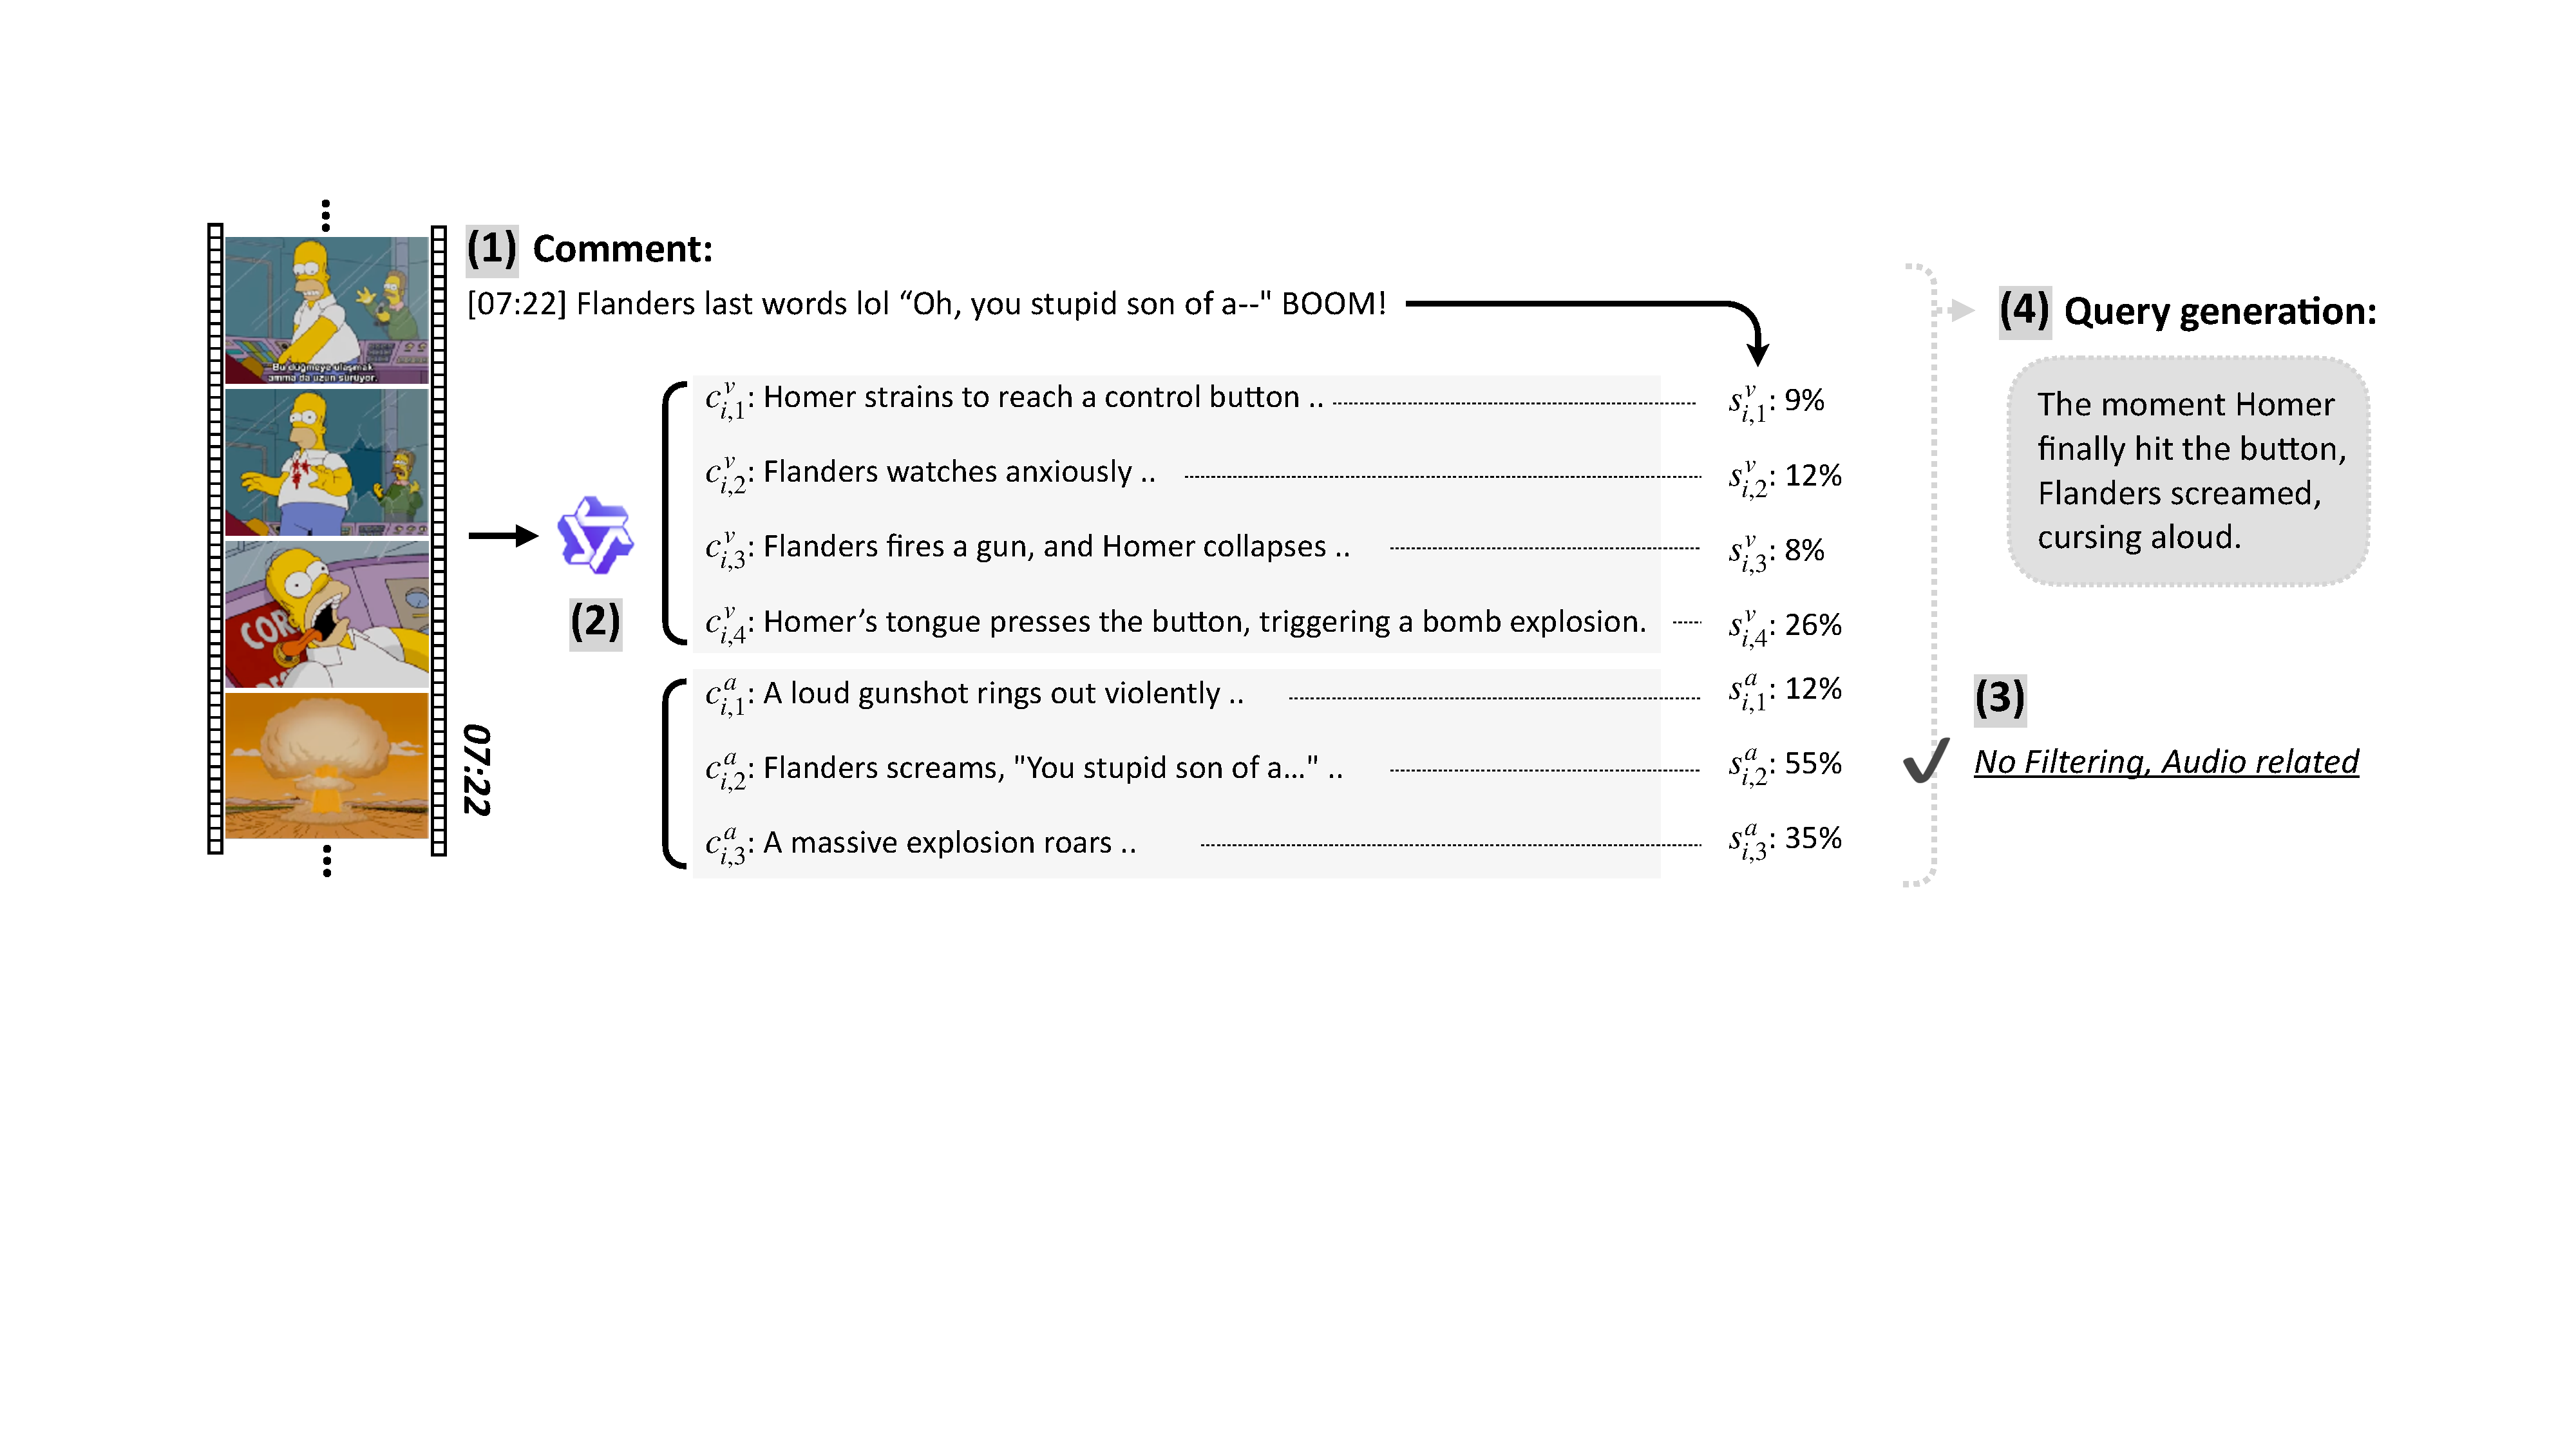
\includegraphics[width=\textwidth]{image/tcvp_overview.pdf}
  }
  \vspace{-1.em}
  \caption{TCVP overview of comment filtering \& modality gating and query generation. TCVP computes comment--caption similarity scores and applies modality gating and then generates a query for the target moment.}
  \label{fig:generation}
% \vspace{-.5em}
\end{figure*}
\paragraph{VMR Dataset Generation}   
Existing work on VMR datasets can be divided into human-annotated and machine-generated approaches. 
Human-annotated datasets~\cite{gao2017tall, lei2020tvr, momentseeker} are constructed by asking annotators to \textit{briefly} watch videos, write a search query, and then localize the corresponding temporal moment.
Specifically, QVHighlights~\cite{QVHighlights} is constructed by asking annotators to write a query for each video and mark the matching time spans and rate how important each clip is for that query. 
Machine-generated datasets typically segment videos into multiple clips according to abrupt changes in visual or audio content, treating all resulting segments as sampled (which we regard as effectively \textit{random}). 
Captions are then generated for each clip to serve as user queries, with recent work such as Watch\&Listen leveraging large language models (LLMs)~\cite{longvale2025,watchandlisten}.

\paragraph{Current Limitations}
Despite such advances in VMR datasets, we identify several limitations in existing pipelines.
In human-annotated settings~\cite{gao2017tall, QVHighlights, momentseeker}, annotators are typically constrained by limited time budgets, which hinders thorough viewing of a video and the selection of moments corresponding to globally important or truly salient events.
In machine-generated approaches~\cite{longvale2025, watchandlisten}, most segments from a long video are adopted regardless of their importance. 
As a result, the moments in the dataset may differ from those that real viewers would want to retrieve. 
Furthermore, the search queries are produced without access to prior knowledge about real user intent. 
This straightforward generation process often results in queries that are overly descriptive, as shown in \figref{fig:pipeline}.
Finally, several studies~\cite{momentseeker} rely exclusively on visual information. However, an analysis of YouTube comments in YTCommentQA~\cite{yang2024ytcommentqa} reveals that about half of user comments refer to audio content. VMR datasets built solely on visual cues therefore fail to capture this substantial portion of user behavior.
% Such datasets may not be beneficial for improving the VMR ability during model training and may not be optimal for reliable model evaluation. This highlights the need for new ideas and pipelines.
Such datasets may not effectively support VMR model training or reliable model evaluation. 
This highlights the need for new ideas and pipelines.

\vspace{+2em}
\section{TCVP: Timestamped Comment-guided VMR Pipeline} 
We present a novel idea to leverage timestamped YouTube comments, which contain both an important moment and real user intent.
% However, directly using comments is challenging because many are uninformative and they often do not show whether the reaction is to what the viewer saw or to what the viewer heard. This makes the user intent unclear.
A naive use of such comments, however, introduces several challenges. First, many comments are uninformative—for example, generic reactions such as ``lol" or ``this is amazing,".
Second, user comments may rely on different modalities, such as visual or audio information, and these comments require distinct data construction procedures.
To address these issues, we propose a realistic VMR dataset generation pipeline, named \textbf{TCVP}.
\figref{fig:generation} illustrates the pipeline, which proceeds through (1) videos and comments collection, (2) modality specific captioning, (3) comment filtering \& modality gating, and (4) query generation.

\vspace{+1.em}
\subsection{Collecting videos and comments}
% \vspace{+3em}
\begin{table}[t]
  \caption{Categories and channels used in our dataset.}
  \centering
  \setlength{\tabcolsep}{4pt}
  \resizebox{\linewidth}{!}{
    \begin{tabular}{l l}
      \hline
      \rowcolor[gray]{0.9}
      \textbf{Category} & \textbf{Channels} \\
      \hline
      \textbf{Knowledge / Education} & TED, BigThink, Kurzgesagt, Veritasium, Vsauce \\
      \textbf{Science / Analysis} & RealLifeLore, WendoverProductions, Vox \\
      \textbf{Documentary} & NatGeo \\
      \textbf{Podcast (Long-form)} & HubermanLab, LexFridman, joerogan, TimFerriss \\
      \textbf{Debate} & OxfordUnion \\
      \textbf{Political Commentary} & LastWeekTonight, TheDailyShow \\
      \textbf{News} & PhilipDeFranco, TheYoungTurks, DWNews \\
      
      % ----------- MULTIROW 1 -----------
      \multirow[t]{2}{*}{\textbf{Talk Show}} 
        & LateNightSeth, JimmyKimmelLive, \\
        & OfficialGrahamNorton, fallontonight \\
      % ---------------------------------
      
      \textbf{Variety / Entertainment} & MrBeast, TopGear \\
      \textbf{Travel / Lifestyle} & KaraandNate, AbroadinJapan, YesTheory \\
      \textbf{Culture / Society} & Jolly, AsianBoss, GeographyNow \\
      \textbf{Cooking / Food} & bingingwithbabish, bonappetit, aragusea \\
      
      % ----------- MULTIROW 2 -----------
      \multirow[t]{2}{*}{\textbf{Making / Engineering}}
        & MarkRober, SmarterEveryDay, \\
        & primitivedechnology9550, Corridor \\
      % ---------------------------------
      
      \textbf{Technology / Tech Review} & TechLead, mkbhd, LinusTechTips \\
      \textbf{Art / Design} & ProkoTV, theartassignment \\
      \textbf{Fashion} & bestdressed, HauteLeMode, Vogue \\
      \textbf{Sports} & NBA, fifa, Olympics \\
      \textbf{Gaming} & PewDiePie, markiplier, pokimane, LoLEsports \\
      \textbf{Comedy / Sketch} & SaturdayNightLive, KeyandPeele \\
      \hline
    \end{tabular}
  }
  \label{tab:video-categories}
\vspace{1.em}
\end{table}

\vspace{+.5em}
We collect videos from Youtube channels listed in Table~\ref{tab:video-categories}, focusing on channels with more than one million subscribers. Such channels host contents that are widely viewed and contain sufficient user comments. For each video, we crawl all comments and retain only those that include timestamps. When multiple comments share the same timestamp, we deduplicate by retaining only the single most-liked comment per timestamp, as the reaction reflects viewer intent at that moment. We then sort these timestamped comments by the number of likes, as likes indicate that many viewers regard the moment as important. For each video, we keep the top 20 timestamped comments and use them in the next steps.

% We collect videos from Youtube channels listed in Table~\ref{tab:video-categories}, focusing on channels with more than one million subscribers. Such channels host contents that are widely viewed and contain sufficient user comments. For each video, we crawl all comments and retain only those that include timestamps. We then sort these timestamped comments by the number of likes, as likes indicate that many viewers regard the moment as important. For each video, we keep the top 20 timestamped comments and use them in the next steps.

\subsection{Modality specific captioning}
\vspace{+.5em}
For each timestamped comment $u_i$, we perform modality-specific captioning.
Specifically, we prompt Qwen2.5-Omni~\cite{qwen2.5omni} to generate short sentences of at most 20 words, producing both visual and audio captions for a 9-second window before and after the timestamp.
% We denote the resulting caption sets as ${c_{i,k}^v}$ and ${c_{i,k}^a}$, respectively, as illustrated in \figref{fig:generation}.
We denote the resulting visual and audio caption sets as ${c_{i,k}^v}$ and  ${c_{i,k}^a}$, respectively, as illustrated in \figref{fig:generation}.
% We adopt a symmetric $[-9\mathrm{s}, +9\mathrm{s}]$ window centered at each timestamp. 
% The empirical justification is provided in Appendix~\ref{sec:ablation_appendix}.
We adopt a symmetric $[-9\mathrm{s}, +9\mathrm{s}]$ window centered at each timestamp, which achieves 97\% moment coverage while larger windows yield diminishing returns (see Appendix~\ref{sec:ablation_appendix}).  
          
% For each timestamped comment $u_i$, we perform modality-specific captioning.
% Specifically, we prompt Qwen2.5-Omni~\cite{qwen2.5omni} to generate short sentences of at most 20 words, producing both visual and audio captions for a 9-second window before and after the timestamp. 
% We denote the resulting caption sets as ${c_{i,k}^v}$ and ${c_{i,k}^a}$, respectively, as illustrated in \figref{fig:generation}.
% The motivation for short sentences is discussed in the following section.

\subsection{Comment filtering \& Modality gating}
\vspace{+.5em}
As noted above, directly using the collected timestamped comments can introduce several issues.
To mitigate these issues, we first introduce a comment filtering mechanism to reduce vague or uninformative comments.
To determine whether a comment contains information relevant to the video content, for each timestamped comment, we compute similarity scores with both visual and audio caption sentences generated in the surrounding temporal window.
The similarity between the comment $u_i$ and the $k$-th visual or audio caption sentence is defined as:
\begin{equation}
\resizebox{0.85\linewidth}{!}{$
s_{i,k}^v=\mathrm{Sim}\left(u_i, c_{i,k}^v\right),
\quad
s_{i,k}^a=\mathrm{Sim}\left(u_i, c_{i,k}^a\right).
$}
\end{equation}
where $\mathrm{Sim}(\cdot,\cdot)$ denotes the cosine similarity computed in the embedding space from the Qwen-3 embedding model.
The maximum similarity for each modality can refer to:
\begin{equation}
s_i^v=\max_k s_{i,k}^v,
\quad
s_i^a=\max_k s_{i,k}^a.
\end{equation}
If $\max(s_i^v, s_i^a)$ is below a predefined threshold $\tau$, we label the comment as unrelated and discard it. In our experiments, we set $\tau = 0.3$.
We observe that overly long caption sentences $c_{i,k}^v \,\text{ or }\, c_{i,k}^a$ tend to yield low similarity scores, as the collected comments are typically short (around 20 words), and we mitigate this issue by encouraging concise captions in the captioning stage.

After comment filtering, we assign each comment to either the visual or audio modality.
Using the maximum similarity scores computed for visual and audio captions, we determine the dominant modality for each comment. Formally, the modality assignment is defined as:
\begin{equation}
\resizebox{0.8\linewidth}{!}{$
m_i=
\begin{cases}
\mathrm{unrelated} & \text{if } \max(s_i^v, s_i^a) < \tau, \\
\mathrm{vision\mbox{-}related} & \text{if } s_i^v \ge s_i^a, \\
\mathrm{audio\mbox{-}related} & \text{if } s_i^a > s_i^v.
\end{cases}
$}
\end{equation}
This modality gating step enables subsequent stages to apply modality-specific processing for moment grounding and query generation.

Figure~\ref{fig:generation} shows an example of modality gating.
% The comment at 07:22 contains a quoted line and yields a higher similarity score with audio captions ($55\%$) than with visual captions ($26\%$), and is therefore assigned to the audio modality and passed to the next stage.
The comment at 07:22 contains a quoted line and yields a higher similarity score with audio captions ($s_{i,2}^a = 55\%$) than with visual captions ($s_{i,4}^v = 26\%$), and is therefore assigned to the audio modality and passed to the next stage. 

\vspace{+2.em}
\subsection{User query generation}
\begin{figure}[t]
  \vspace{1em}
  \centering
  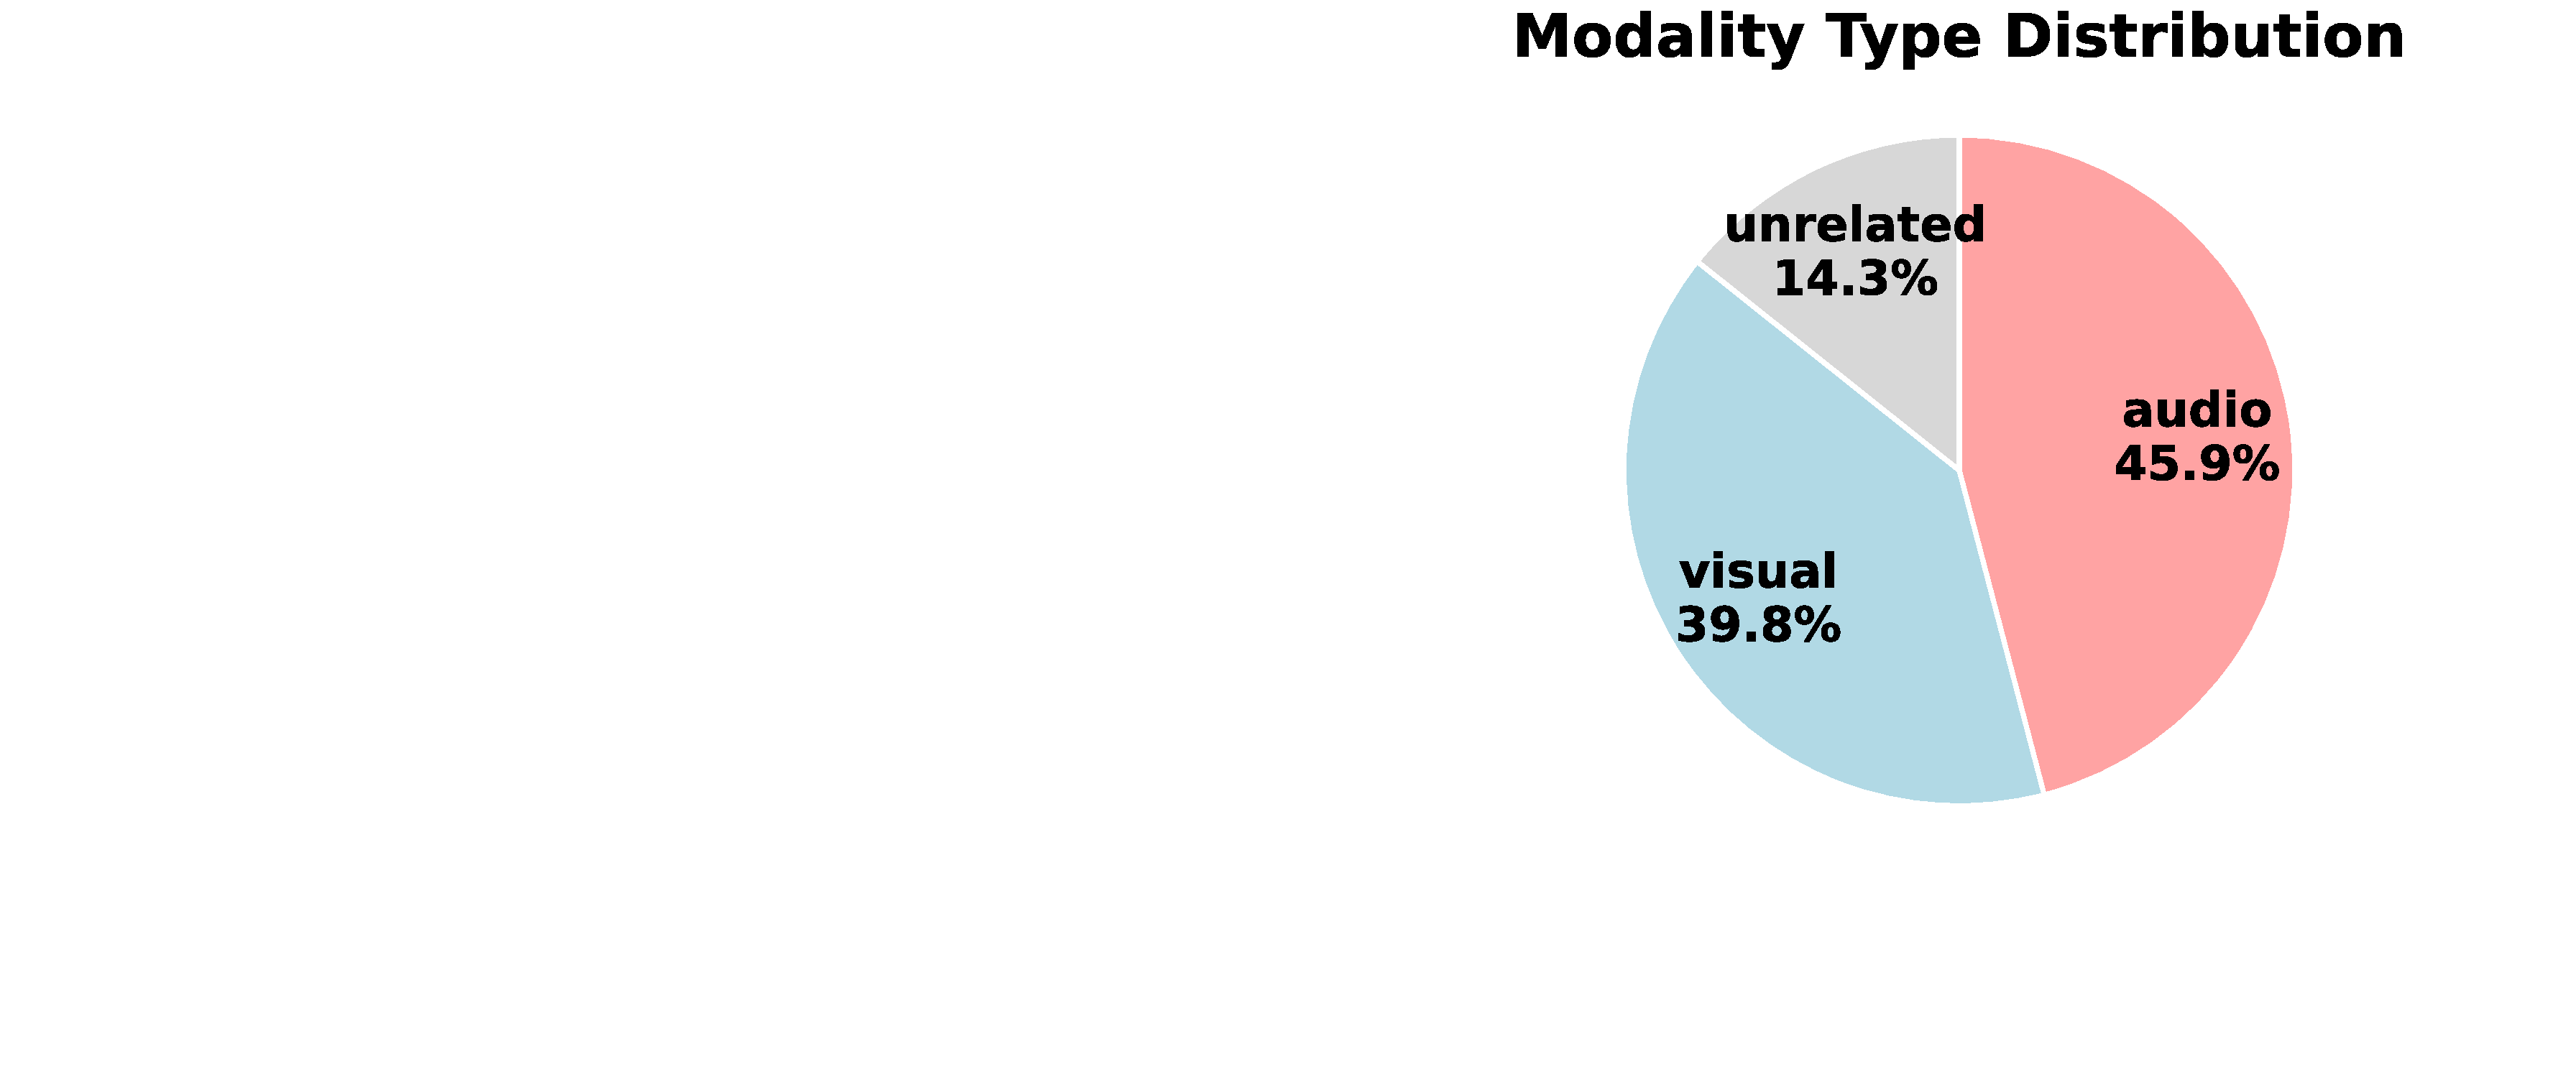
\includegraphics[width=0.65\linewidth]{image/modality_stat.pdf}
  \caption{Dataset statistics for modality. The pie chart shows the overall split of visual-related, audio-related, and unrelated comments.}
  \label{fig:stat}
  \vspace{-1em}
\end{figure}
% In this step, we generate user queries $q_i$ by leveraging the information collected in the previous stages.
By grounding query generation in the timestamped comment itself, we ensure that each $q_i$ captures real user intent and key expressions rather than generic video descriptions. 
Specifically, we prompt GPT-4.1~\citep{openai_gpt41} with the comment and modality-specific captions, instructing it to extract keywords directly from the comment and formulate a natural, search-oriented query. 
Query generation is conditioned on the assigned modality, visual captions for vision-related comments and audio captions for audio-related ones, preventing mismatched evidence and grounding each query in the correct modality. 
We release our dataset, including our code, video links, collected comments, modality labels, and user-like queries. The prompts used in our pipeline are provided in the appendix~\ref{sec:generation_prompts}.

% We prompt GPT-4.1~\citep{openai_gpt41} with the timestamped comment and the modality-specific captions to produce a $q_i$.
% Unlike prior approaches, we explicitly instruct the GPT to referring the underlying user intent in user comments and extracting keywords from the comment. 
% The $q_i$ is then formulated based on these keywords to resemble a natural search query rather than a descriptive caption.
% Moreover, query generation is conditioned on the assigned modality, using visual captions for vision-related comments and audio or speech captions for audio-related comments. 
% This prevents the model from relying on mismatched evidence and helps generate queries grounded in the correct modality.

% We will release our dataset, which includes our code, video links, collected comments, modality labels, and user-like queries. 


% We release our dataset, including our code, video links, collected comments, modality labels, and user-like queries. The prompts used in our pipeline are provided in the appendix~\ref{sec:generation_prompts}.             
% A comparison between our dataset and existing VMR datasets is provided in Table~\ref{tab:benchmark_comparison}.

% pdf로 바꾸어서 넣기. 
\begin{figure*}[t]
  \centering
  \resizebox{\linewidth}{!}{
    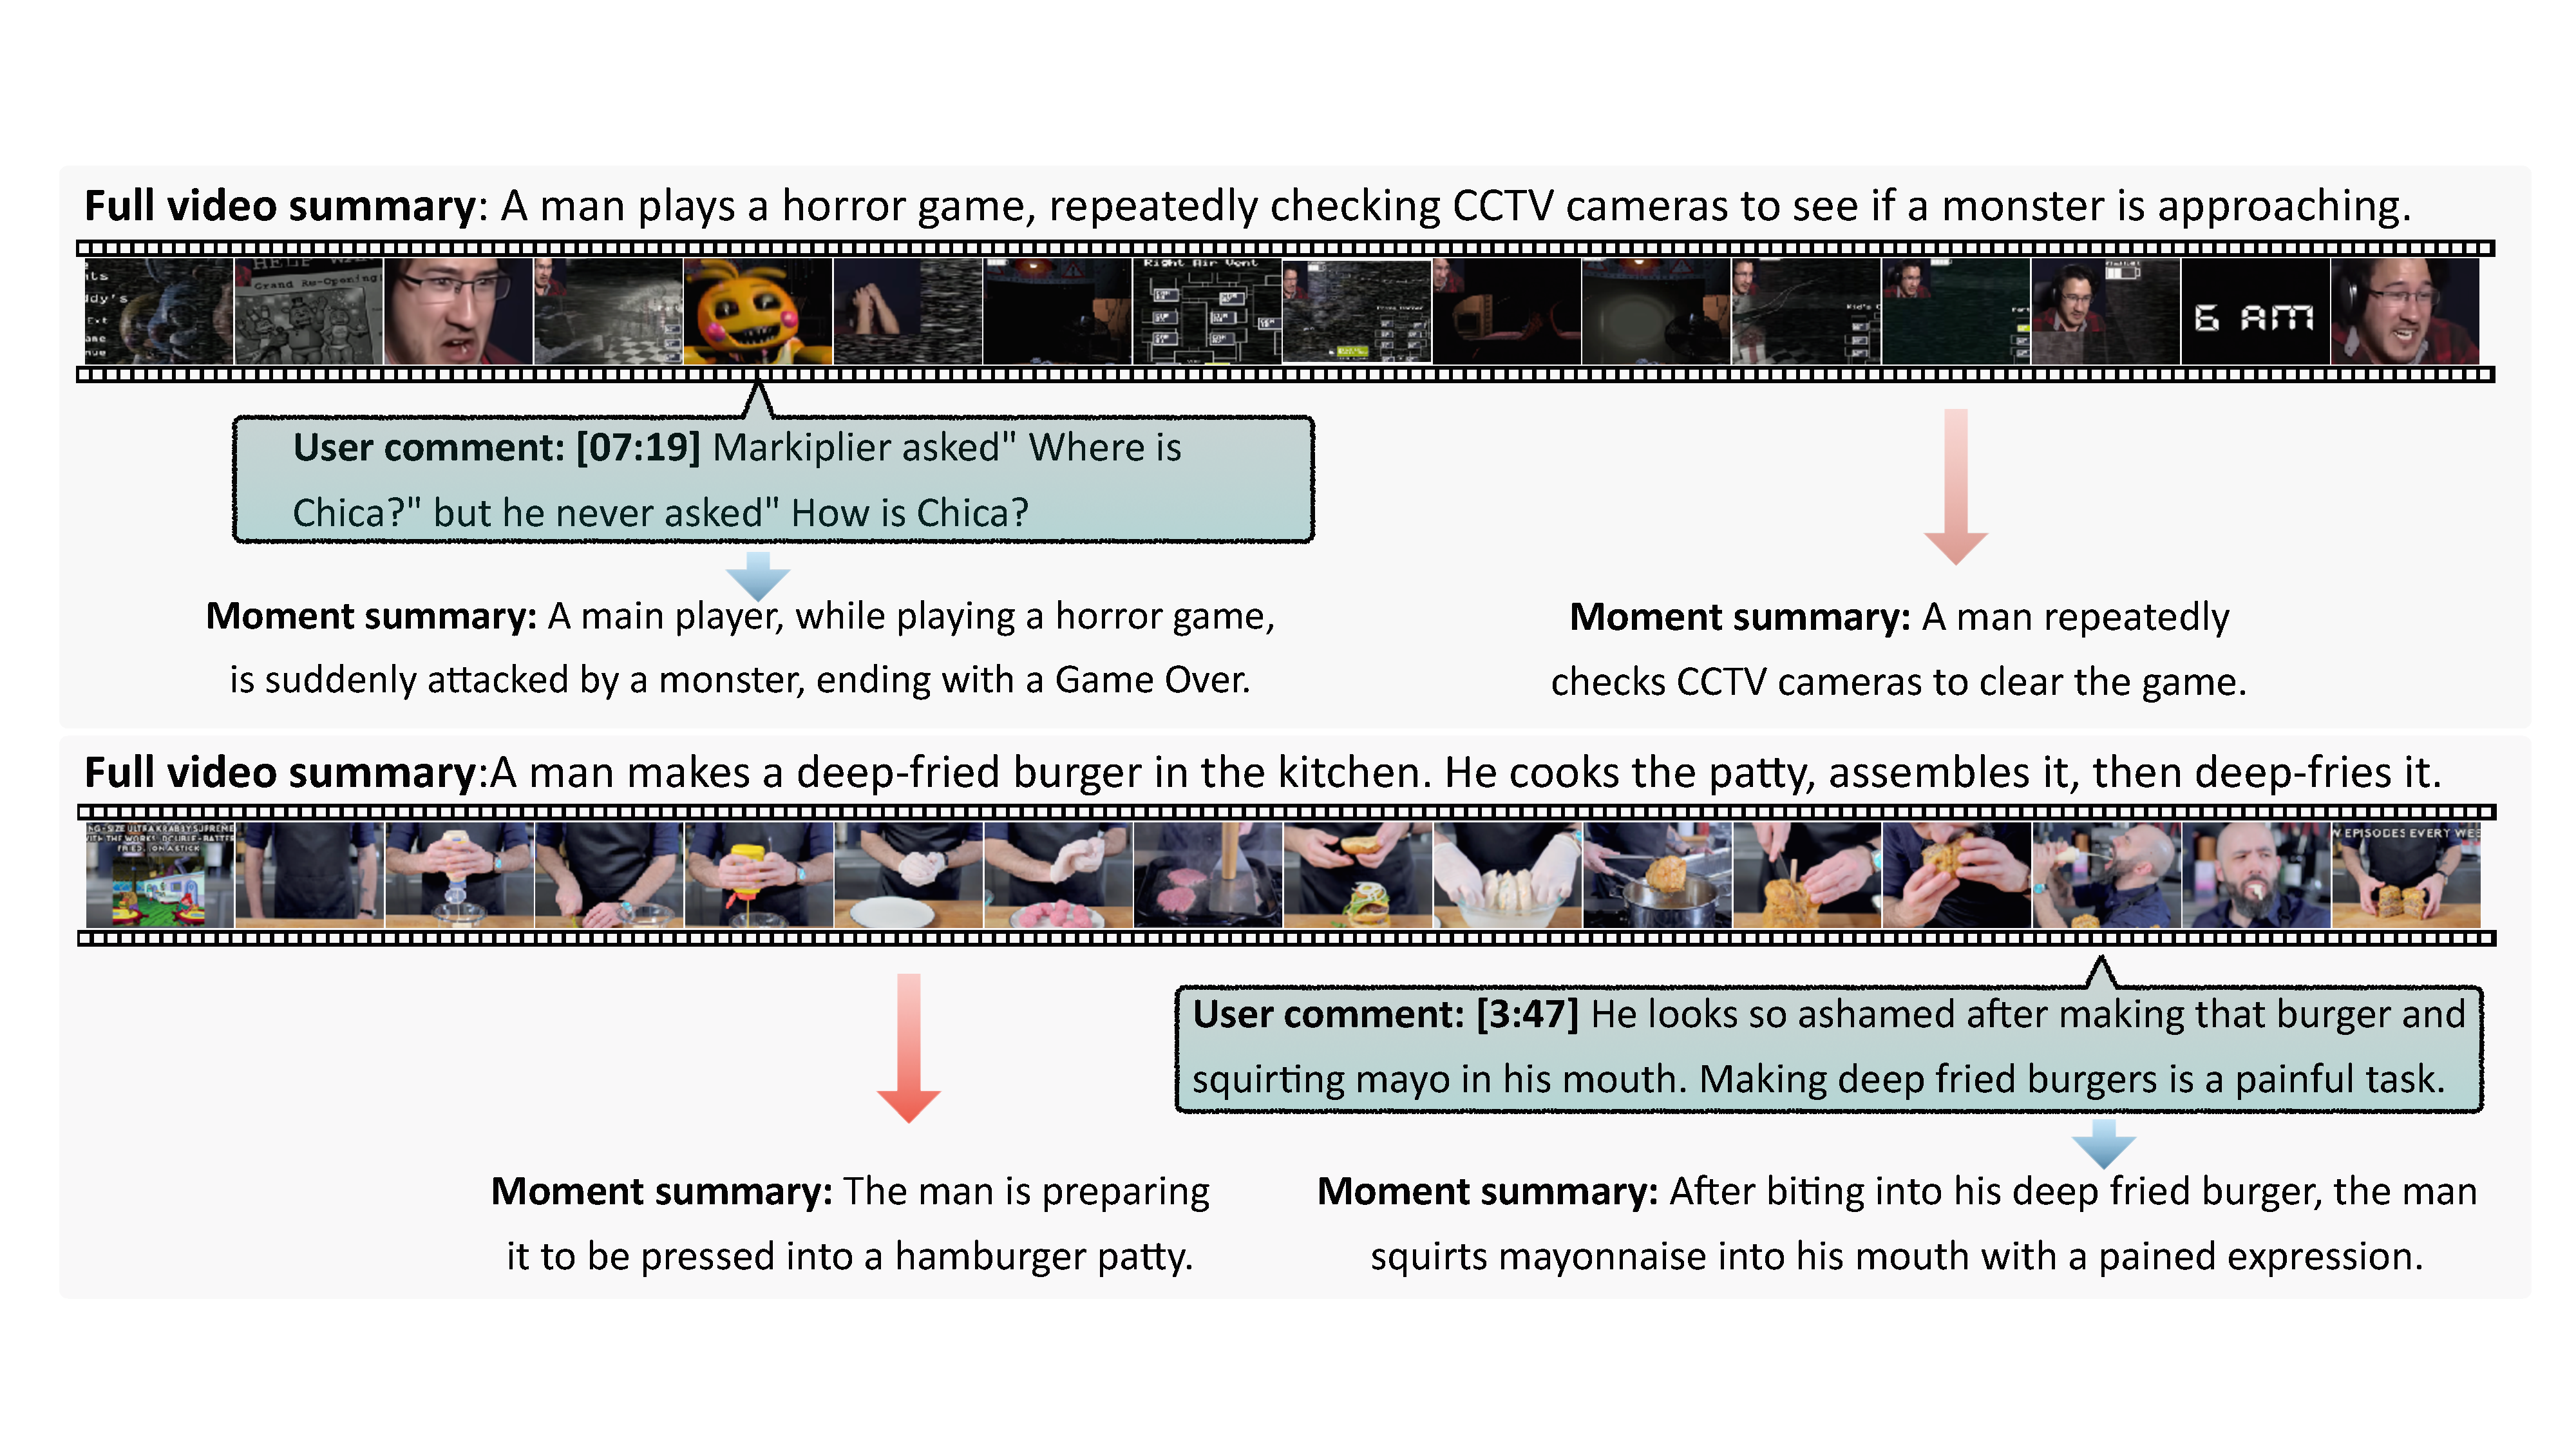
\includegraphics[width=\textwidth]{image/moment_selection_qual.pdf}
  }
  \vspace{-1.5em}
  \caption{Qualitative comparison of moment selection within the same videos. Comment-based selection (timestamped user comments) tends to capture eventful segments that attract user reactions, whereas random sampling often yields ordinary segments with weak retrieval cues.}
  \label{fig:qualitative_result}
  \vspace{-1.em}
\end{figure*}

\section{Analysis of TCVP}

In this section, we analyze our dataset generated by TCVP. 
We examine its modality statistics and conduct a qualitative comparison of both moments and user queries against existing VMR datasets, followed by human evaluation results. 
Detailed evaluation protocols are provided in Appendix~\ref{sec:human_appendix}.

\subsection{Results of our filtering \& gating}
Figure~\ref{fig:stat} reports the results after applying the third stage of our pipeline.
Overall, 45.9\% of comments are labeled as audio-related and 39.8\% as vision-related, while 14.3\% are filtered out as unrelated.
The results show that many comments point to audio or speech cues, aligning with findings from YT-CommentQA~\cite{yang2024ytcommentqa} discussed in \secref{sec:section2}.
This underscores the importance of audio modeling for realistic VMR datasets.
We set $\tau\!=\!0.3$, which retains semantically grounded comments (\eg, ``insane goal at the last second'') while filtering generic reactions (\eg, ``lol''); sensitivity analysis is provided in Appendix~\ref{sec:ablation_appendix}.             

% The effect of varying $\tau$ on the modality distribution is reported in Appendix~\ref{sec:ablation_appendix}.

\subsection{Qualitative comparison of moment selection}
Figure~\ref{fig:qualitative_result} compares moments selected at comment timestamps with random selection from the same videos.
In the horror gameplay video shown in \figref{fig:qualitative_result}, the comment-aligned moment captures a sudden monster attack that results in a game over, whereas the randomly selected moment (\eg, red arrow) depicts the player checking CCTV cameras, which is less relevant to viewer interest.
In the cooking video, the random moment captures a routine preparation action (\eg, pressing a patty) with limited distinctive retrieval cues.
We further present a human evaluation on moment selection in the following subsection.



\subsection{Human evaluation: Timestamped moment vs. randomly selected moment}
We randomly select 40 samples balanced across all video categories, yielding 120 total assessments per task.
For each sample, annotators compare two candidate moments, one from timestamped comments and one from random sampling, and choose the moment that is more likely to be searched to retrieve.
Judgments from three independent annotators are aggregated by majority vote.
Figure~\ref{fig:moment_survey} shows that annotators prefer comment-based selection in 95\% of videos, while random sampling is preferred in 5\%.
These results demonstrate that timestamped comments are effective signals for identifying moments that align with user search intent.

\begin{figure}[t]
    \centering
      \resizebox{0.9\linewidth}{!}{
        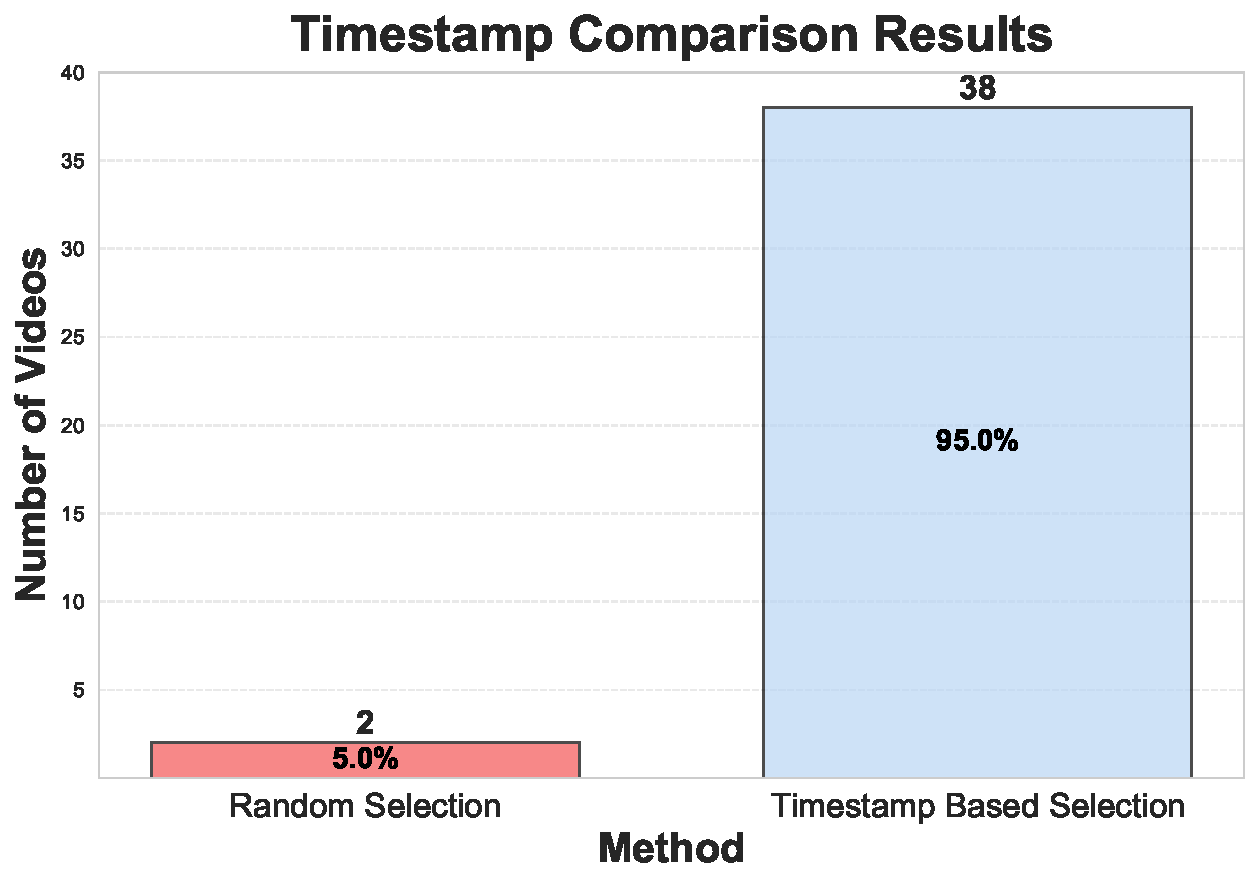
\includegraphics{image/moment_human_eval.pdf}
      }
      \vspace{-.5em}
    \caption{Human evaluation of moment selection. Annotators choose the moment that is more likely to be searched for retrieval between comment-based selection and random sampling.}
    \label{fig:moment_survey}
    \vspace{-1em}
\end{figure}

% pdf로 바꾸어서 넣기. 
\begin{figure*}[t]
  \centering
  \resizebox{\linewidth}{!}{
    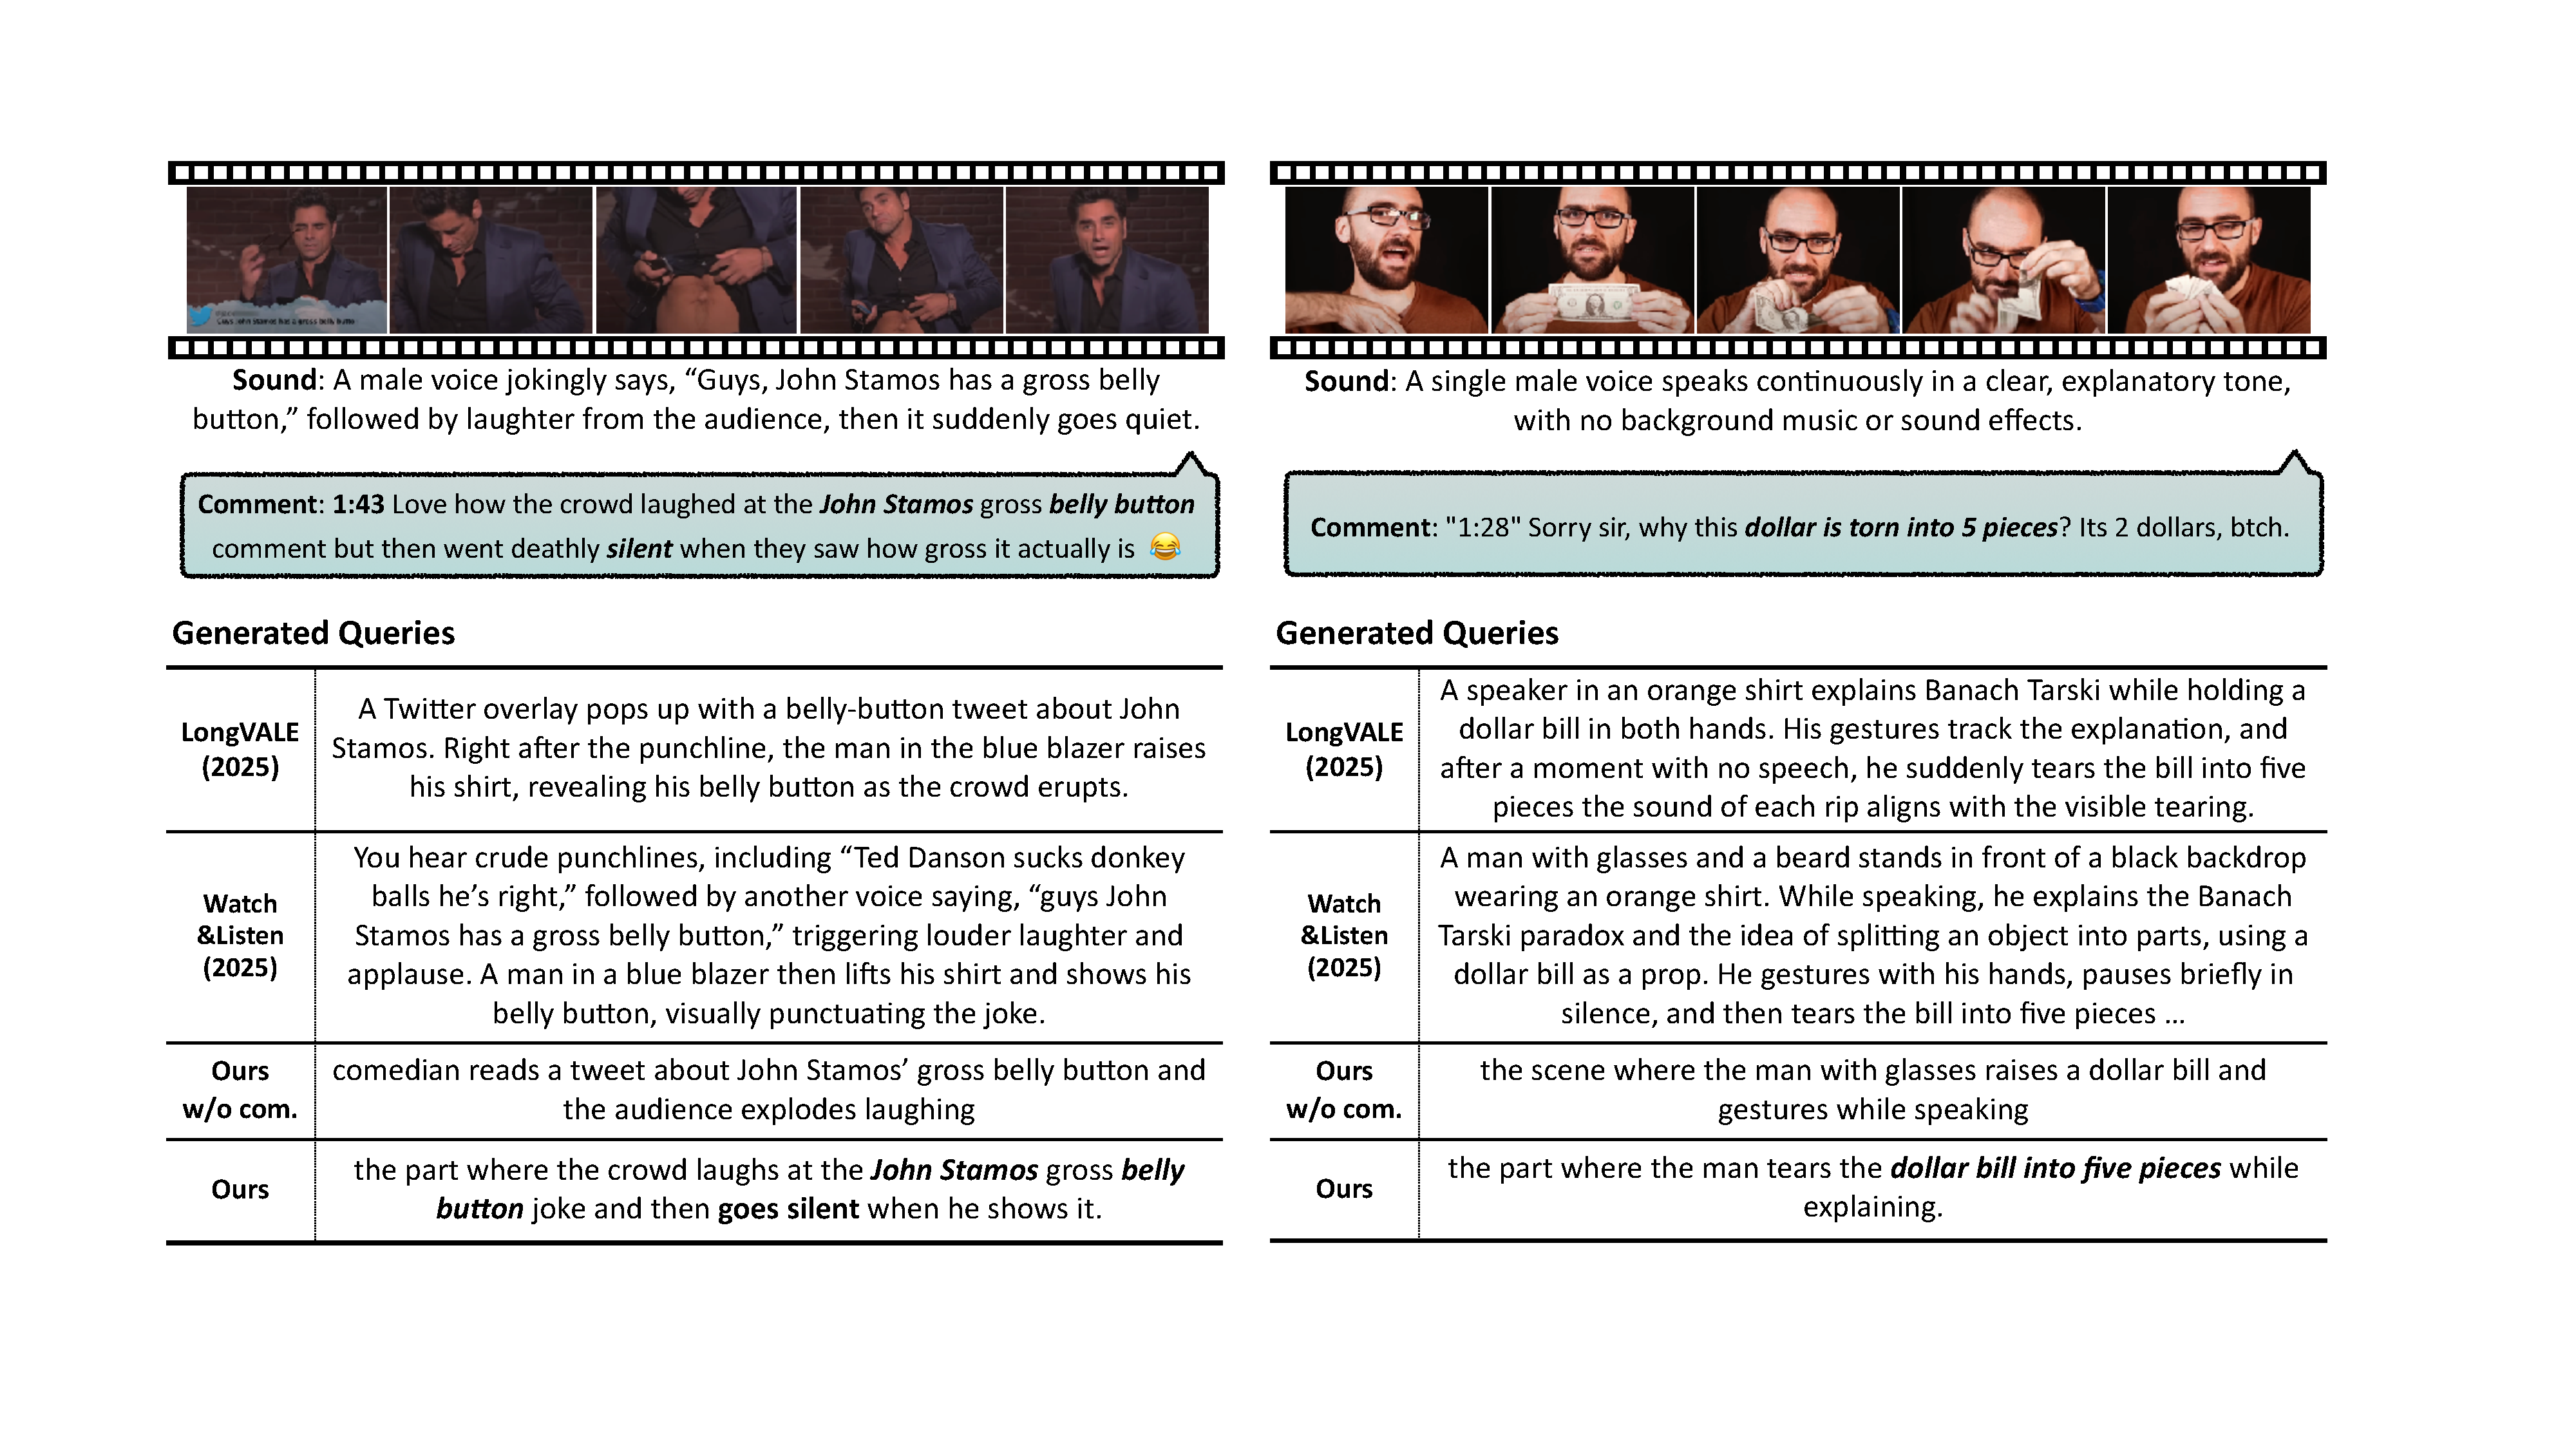
\includegraphics[width=\textwidth]{image/query_gen_qual.pdf}
  }
  \vspace{-1.5em}
  \caption{Qualitative comparison of queries generated for the same moments. Each example shows sampled frames, an audio summary, and the anchor timestamped comment, followed by queries from caption-based baselines (LongVALE, Watch\&Listen) and our variants (ours w/o comments and ours w/ comments).}
  \vspace{-1em}
  \label{fig:query_qualitative_result}
\end{figure*}

\subsection{Qualitative comparison of user queries}
An example in Figure~\ref{fig:query_qualitative_result} shows a timestamped comment querying the reason a dollar bill is torn into five pieces, with the corresponding clip depicting the speaker explaining the action.
In LongVALE and Watch\&Listen, the query is driven by broad clip descriptions, remaining tied to the lecture context and incorporating peripheral details (e.g., the Banach–Tarski explanation).
Without the comment (\ie, ours w/o com.), the query stays at a generic description such as holding the bill and speaking, so the key action that viewers want to retrieve is not singled out.
In contrast, conditioning on the timestamped comment (\ie, ours) yields a query directly targets the bill being torn into five pieces, closely reflecting the underlying user intent.

\subsection{Human evaluation: are our queries realistic?}
To support the qualitative comparison, we conduct a human evaluation study that assesses the naturalness and realism of the queries.
The instruction can found in \figref{fig:query_survey}. 
Annotators see four candidates from LongVALE, Watch\&Listen, Ours w/o comments, and Ours w/ comments, and they select the best one, with three independent judgments aggregated by majority vote.
Figure~\ref{fig:query survey result} shows that \textbf{Ours w/ comments} is preferred in 70\% of cases and \textbf{Ours w/o comments} in 25\%, while LongVALE accounts for 5\% and Watch\&Listen is never selected. 
This result indicates that leveraging timestamped comments improves both the naturalness and realism of the generated queries.


\begin{figure}[t]
    \centering
      \resizebox{0.9\linewidth}{!}{
        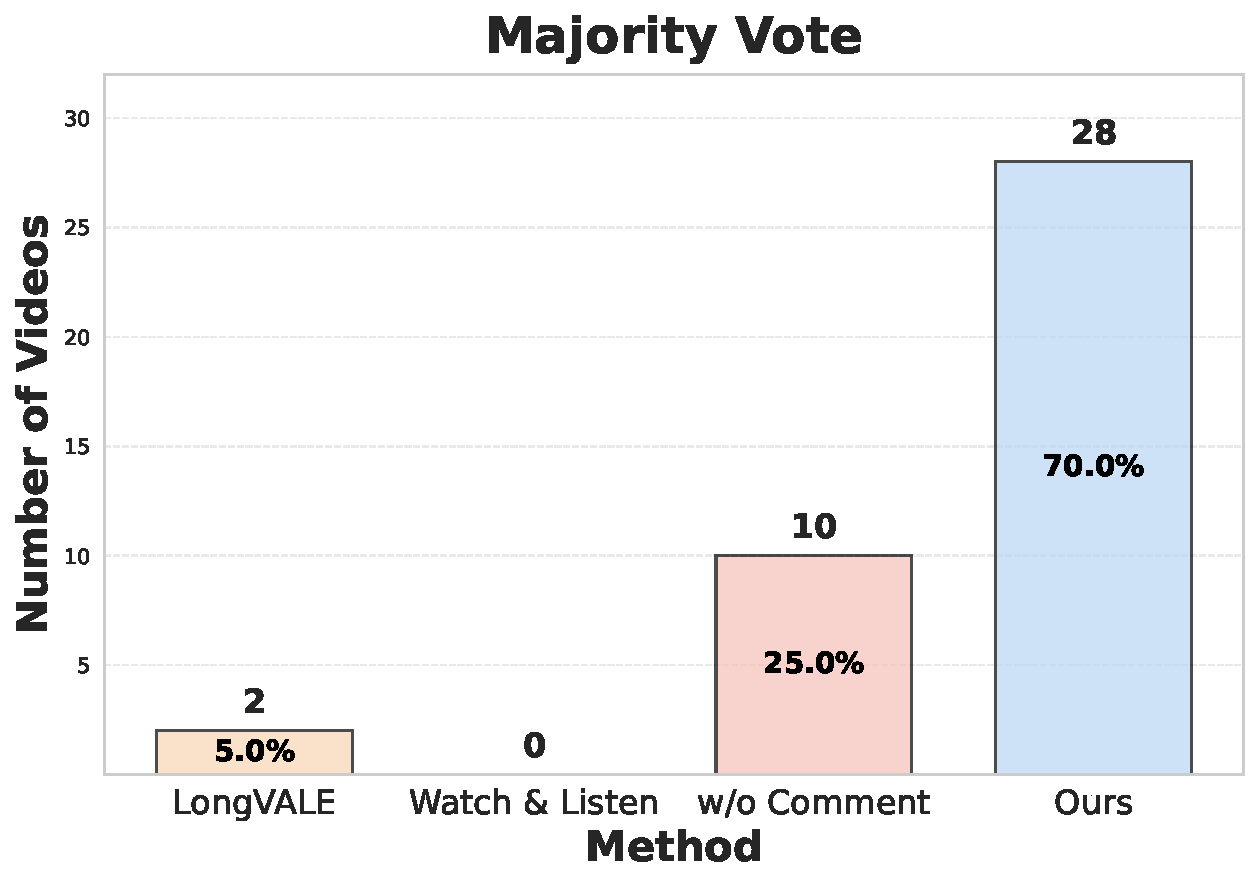
\includegraphics{image/query_human_eval.pdf}
      }
    \vspace{-.5em}
    \caption{Human evaluation of generated queries. We compare caption-based baselines (LongVALE, Watch\&Listen) with our dataset.}
    \vspace{-1em}

    \label{fig:query survey result}
\end{figure}



% \begin{table*}[t]
%   \centering
%   \small
%   \renewcommand{\arraystretch}{1.15}
%   \begin{tabular}{lccccc cccccc}
%     \toprule
%     \multirow{2}{*}{\textbf{Model}} &
%     \multirow{2}{*}{\textbf{Size}} &
%     \multicolumn{3}{c}{\textbf{Input modality}} &
%     \multicolumn{2}{c}{\textbf{visual-related}} &
%     \multicolumn{2}{c}{\textbf{audio-related}} &
%     \multicolumn{2}{c}{\textbf{mixed-related}} \\
%     \cmidrule(lr){3-5}
%     \cmidrule(lr){6-7}
%     \cmidrule(lr){8-9}
%     \cmidrule(lr){10-11}
%       &  & \textbf{V} & \textbf{A} & \textbf{ASR} 
%       & \textbf{R@1} & \textbf{mAP}
%       & \textbf{R@1} & \textbf{mAP}
%       & \textbf{R@1} & \textbf{mAP} \\
%     \midrule

%     \multicolumn{11}{c}{\textbf{Closed-source models}} \\
%     \midrule
%     Gemini 2.5 Pro~\cite{gemini25pro} 
%                     & -- & $\checkmark$ & $\checkmark$ & $\checkmark$
%                     & \textemdash & \textemdash & \textemdash & \textemdash & \textemdash & \textemdash \\
%     GPT\mbox{-}4o~\cite{gpt4o}
%                     & -- & $\checkmark$ & $\checkmark$ & $\checkmark$
%                     & \textemdash & \textemdash & \textemdash & \textemdash & \textemdash & \textemdash \\
%     \midrule

%     \multicolumn{11}{c}{\textbf{Open-source models}} \\
%     \midrule
%     Qwen2.5-Omni~\cite{qwen25omni} 
%                     & 7B & $\checkmark$ & $\checkmark$ & $\checkmark$
%                     & \textemdash & \textemdash & \textemdash & \textemdash & \textemdash & \textemdash \\
%     Qwen2.5-VL~\cite{qwen25vl}
%                     & 7B & $\checkmark$ & $\times$     & $\times$
%                     & \textemdash & \textemdash & \textemdash & \textemdash & \textemdash & \textemdash \\
%     Qwen2.5-VL~\cite{qwen25vl}
%                     & 7B & $\checkmark$ & $\times$     & $\checkmark$
%                     & \textemdash & \textemdash & \textemdash & \textemdash & \textemdash & \textemdash \\                    
%     InternVL3.5~\cite{internvl35}
%                     & 8B & $\checkmark$ & $\times$     & $\times$
%                     & \textemdash & \textemdash & \textemdash & \textemdash & \textemdash & \textemdash \\
%     InternVL3.5~\cite{internvl35}
%                     & 8B & $\checkmark$ & $\times$     & $\checkmark$
%                     & \textemdash & \textemdash & \textemdash & \textemdash & \textemdash & \textemdash \\             
%     \midrule
%     \multicolumn{11}{c}{\textbf{Video Retrieval Models}} \\
%     \midrule
%     Qwen2.5-Omni~\cite{qwen25omni} 
%                     & 7B & $\checkmark$ & $\checkmark$ & $\checkmark$
%                     & \textemdash & \textemdash & \textemdash & \textemdash & \textemdash & \textemdash \\
%     Qwen2.5-VL~\cite{qwen25vl}
%                     & 7B & $\checkmark$ & $\times$     & $\times$
%                     & \textemdash & \textemdash & \textemdash & \textemdash & \textemdash & \textemdash \\
%     Qwen2.5-VL~\cite{qwen25vl}
%                     & 7B & $\checkmark$ & $\times$     & $\checkmark$
%                     & \textemdash & \textemdash & \textemdash & \textemdash & \textemdash & \textemdash \\                    
%     InternVL3.5~\cite{internvl35}
%                     & 8B & $\checkmark$ & $\times$     & $\times$
%                     & \textemdash & \textemdash & \textemdash & \textemdash & \textemdash & \textemdash \\
%     InternVL3.5~\cite{internvl35}
%                     & 8B & $\checkmark$ & $\times$     & $\checkmark$
%                     & \textemdash & \textemdash & \textemdash & \textemdash & \textemdash & \textemdash \\                       
%     \bottomrule
%   \end{tabular}
%   \caption{Comparison across models, input modality configurations, and query types. 
%   Closed-source and open-source models are shown separately for clarity.}
%   \label{tab:mllm-eval-result}
% \end{table*}


% \begin{table*}[t]
%   \centering
%   \caption{Comparison across models, input modality configurations, and query types.}
%   \setlength{\tabcolsep}{8pt}
%   \resizebox{0.8\linewidth}{!}{
%     \begin{tabular}{l c c c c c c c c c c}
%       \hline
%       \rowcolor[gray]{0.9}
%       \multirow[t]{2}{*}{\textbf{Model}} &
%       \multirow[t]{2}{*}{\textbf{Size}} &
%       \multicolumn{3}{c}{\textbf{Input modality}} &
%       \multicolumn{2}{c}{\textbf{visual}} &
%       \multicolumn{2}{c}{\textbf{audio}} &
%       \multicolumn{2}{c}{\textbf{mixed}} \\
%       \rowcolor[gray]{0.9}
%       & & \textbf{V} & \textbf{A} & \textbf{ASR}
%       & \textbf{R@1} & \textbf{mAP}
%       & \textbf{R@1} & \textbf{mAP}
%       & \textbf{R@1} & \textbf{mAP} \\
%       \hline

%       % ---------------- CLOSED SOURCE ----------------
%       \rowcolor[gray]{0.95}
%       \multicolumn{11}{l}{\textbf{Closed-source models}} \\
%       Gemini 2.5 Pro~\cite{gemini25pro}
%         & -- & \cmark & \cmark & \cmark
%         & --- & --- & --- & --- & --- & --- \\
%       GPT\mbox{-}4o~\cite{gpt4o}
%         & -- & \cmark & \cmark & \cmark
%         & --- & --- & --- & --- & --- & --- \\
%       \hline

%       % ---------------- OPEN SOURCE ----------------
%       \rowcolor[gray]{0.95}
%       \multicolumn{11}{l}{\textbf{Open-source models}} \\
%       Qwen2.5-Omni~\cite{qwen25omni}
%         & 7B & \cmark & \cmark & \cmark
%         & --- & --- & --- & --- & --- & --- \\
%       Qwen2.5-VL~\cite{qwen25vl}
%         & 7B & \cmark & \xmark & \xmark
%         & --- & --- & --- & --- & --- & --- \\
%       Qwen2.5-VL~\cite{qwen25vl}
%         & 7B & \cmark & \xmark & \cmark
%         & --- & --- & --- & --- & --- & --- \\
%       InternVL3.5~\cite{internvl35}
%         & 8B & \cmark & \xmark & \xmark
%         & --- & --- & --- & --- & --- & --- \\
%       InternVL3.5~\cite{internvl35}
%         & 8B & \cmark & \xmark & \cmark
%         & --- & --- & --- & --- & --- & --- \\
%       \hline

%       % ---------------- VIDEO RETRIEVAL MODELS ----------------
%       \rowcolor[gray]{0.95}
%       \multicolumn{11}{l}{\textbf{Video Retrieval Models}} \\
%       Qwen2.5-Omni~\cite{qwen25omni}
%         & 7B & \cmark & \cmark & \cmark
%         & --- & --- & --- & --- & --- & --- \\
%       Qwen2.5-VL~\cite{qwen25vl}
%         & 7B & \cmark & \xmark & \xmark
%         & --- & --- & --- & --- & --- & --- \\
%       Qwen2.5-VL~\cite{qwen25vl}
%         & 7B & \cmark & \xmark & \cmark
%         & --- & --- & --- & --- & --- & --- \\
%       InternVL3.5~\cite{internvl35}
%         & 8B & \cmark & \xmark & \xmark
%         & --- & --- & --- & --- & --- & --- \\
%       InternVL3.5~\cite{internvl35}
%         & 8B & \cmark & \xmark & \cmark
%         & --- & --- & --- & --- & --- & --- \\
%       \hline
%     \end{tabular}
%   }
%   \label{tab:mllm-eval-result}
% \end{table*}

% \begin{table*}[t]
%   \centering
%   \caption{Comparison of VMR performance across models and input modality configurations,
%   evaluated using Recall@1, Recall@5, and Recall@10.}
%   \setlength{\tabcolsep}{6pt}
%   \resizebox{\linewidth}{!}{
%     \begin{tabular}{l c c c c c c c c c c c c c}
%       \hline
%       \rowcolor[gray]{0.9}
%       \multirow[t]{2}{*}{\textbf{Model}} &
%       \multirow[t]{2}{*}{\textbf{Size}} &
%       \multicolumn{3}{c}{\textbf{Input modality}} &
%       \multicolumn{3}{c}{\textbf{Visual}} &
%       \multicolumn{3}{c}{\textbf{Audio}} &
%       \multicolumn{3}{c}{\textbf{Overall}} \\
%       \rowcolor[gray]{0.9}
%       & & \textbf{V} & \textbf{A} & \textbf{ASR}
%       & \textbf{R@1} & \textbf{R@5} & \textbf{R@10}
%       & \textbf{R@1} & \textbf{R@5} & \textbf{R@10}
%       & \textbf{R@1} & \textbf{R@5} & \textbf{R@10} \\
%       \hline

%       % ---------------- CLOSED SOURCE ----------------
%       \rowcolor[gray]{0.95}
%       \multicolumn{14}{l}{\textbf{Closed-source models}} \\
%       Gemini 2.5 Pro~\cite{gemini25pro}
%         & -- & \cmark & \cmark & \cmark
%         & -- & -- & -- & -- & -- & -- & -- & -- & -- \\
%       GPT\mbox{-}4o~\cite{gpt4o}
%         & -- & \cmark & \cmark & \cmark
%         & -- & -- & -- & -- & -- & -- & -- & -- & -- \\
%       \hline

%       % ---------------- BASELINES ----------------
%       \rowcolor[gray]{0.95}
%       \multicolumn{14}{l}{\textbf{Baselines}} \\
%       Random
%         & -- & -- & -- & --
%         & 1.75 & 9.34 & 20.13
%         & 1.33 & 8.42 & 16.40
%         & 1.51 & 8.62 & 17.58 \\
%       \hline

%       % ---------------- OPEN SOURCE (MLLMs) ----------------
%       \rowcolor[gray]{0.95}
%       \multicolumn{14}{l}{\textbf{Open-source MLLMs}} \\
%       Qwen 2.5 VL-3B
%         & 3B & \cmark & \xmark & \xmark
%         & 6.07 & -- & --
%         & 4.56 & -- & --
%         & 5.26 & -- & -- \\
%       Qwen 2.5 VL-3B-caption
%         & 3B & \cmark & \xmark & \xmark
%         & 7.47 & 22.62 & 33.36
%         & 4.09 & 13.04 & 23.12
%         & 5.04 & 16.07 & 26.20 \\
%       Qwen 2.5 VL-3B-caption + Sub.
%         & 3B & \cmark & \xmark & \cmark
%         & 8.56 & 25.63 & 37.31
%         & 20.51 & 42.69 & 52.63
%         & 13.52 & 31.52 & 41.97 \\
%       \hline

%       Qwen 3 VL-2B
%         & 2B & \cmark & \xmark & \xmark
%         & 3.42 & -- & --
%         & 5.28 & -- & --
%         & 4.42 & -- & -- \\
%       Qwen 3 VL-2B-caption
%         & 2B & \cmark & \xmark & \xmark
%         & 11.47 & 30.18 & 42.42
%         & 4.17 & 14.18 & 24.50
%         & 7.04 & 20.24 & 31.18 \\
%       Qwen 3 VL-2B-caption + Sub.
%         & 2B & \cmark & \xmark & \cmark
%         & 8.68 & 24.80 & 36.69
%         & 20.64 & 40.48 & 50.62
%         & 13.34 & 30.06 & 40.62 \\
%       \hline

%       InternVL3-2B
%         & 2B & \cmark & \xmark & \xmark
%         & 3.68 & -- & --
%         & 2.47 & -- & --
%         & 2.89 & -- & -- \\
%       InternVL3-2B-caption
%         & 2B & \cmark & \xmark & \xmark
%         & 8.59 & 23.61 & 35.09
%         & 3.10 & 11.88 & 22.15
%         & 5.18 & 16.37 & 26.69 \\
%       InternVL3-2B-caption + Sub.
%         & 2B & \cmark & \xmark & \cmark
%         & 8.01 & 23.57 & 35.09
%         & 20.23 & 40.32 & 50.13
%         & 13.25 & 29.78 & 40.04 \\
%       \hline

%       % ---------------- VIDEO RETRIEVAL MODELS ----------------
%       \rowcolor[gray]{0.95}
%       \multicolumn{14}{l}{\textbf{Video Retrieval Models}} \\
%       CLAP
%         & -- & \xmark & \cmark & \xmark
%         & 4.08 & 15.73 & 27.29
%         & 2.30 & 12.69 & 24.22
%         & 3.12 & 14.10 & 25.65 \\
%       LanguageBind-Audio
%         & -- & \xmark & \cmark & \xmark
%         & 3.28 & 15.29 & 27.74
%         & 3.07 & 13.84 & 24.07
%         & 3.16 & 14.51 & 25.77 \\
%       CLIP
%         & -- & \cmark & \xmark & \xmark
%         & 24.83 & 44.88 & 57.04
%         & 11.02 & 24.03 & 35.73
%         & 17.46 & 33.76 & 45.67 \\
%       LanguageBind
%         & -- & \cmark & \xmark & \xmark
%         & 30.54 & 49.97 & 62.72
%         & 14.16 & 26.31 & 37.03
%         & 21.78 & 37.32 & 48.98 \\
%       InternVideo2
%         & -- & \cmark & \xmark & \xmark
%         & 16.54 & 43.00 & 57.90
%         & 5.52 & 19.20 & 31.49
%         & 10.57 & 30.09 & 43.57 \\
%       \hline
%     \end{tabular}
%   }
%   \label{tab:mllm-eval-result}
% \end{table*}



% \begin{table*}[t]
%   \centering
%   \caption{Comparison of VMR performance across models and input modality configurations,
%   evaluated using Recall@1, Recall@5, and Recall@10.}
%   \setlength{\tabcolsep}{6pt}
%   \resizebox{\linewidth}{!}{
%     \begin{tabular}{l c c c c c c c c c c c c c}
%       \hline
%       \rowcolor[gray]{0.9}
%       \multirow[t]{2}{*}{\textbf{Model}} &
%       \multirow[t]{2}{*}{\textbf{Size}} &
%       \multicolumn{3}{c}{\textbf{Input modality}} &
%       \multicolumn{3}{c}{\textbf{Visual}} &
%       \multicolumn{3}{c}{\textbf{Audio}} &
%       \multicolumn{3}{c}{\textbf{Overall}} \\
%       \rowcolor[gray]{0.9}
%       & & \textbf{V} & \textbf{A} & \textbf{ASR}
%       & \textbf{R@1} & \textbf{R@5} & \textbf{R@10}
%       & \textbf{R@1} & \textbf{R@5} & \textbf{R@10}
%       & \textbf{R@1} & \textbf{R@5} & \textbf{R@10} \\
%       \hline

%       % ---------------- CLOSED SOURCE ----------------
%       \rowcolor[gray]{0.95}
%       \multicolumn{14}{l}{\textbf{Closed-source models}} \\
%       Gemini 2.5 Pro~\cite{gemini25pro}
%         & -- & \cmark & \cmark & \cmark
%         & -- & -- & -- & -- & -- & -- & -- & -- & -- \\
%       GPT\mbox{-}4o~\cite{gpt4o}
%         & -- & \cmark & \cmark & \cmark
%         & -- & -- & -- & -- & -- & -- & -- & -- & -- \\
%       \hline

%       % ---------------- BASELINES ----------------
%       \rowcolor[gray]{0.95}
%       \multicolumn{14}{l}{\textbf{Baselines}} \\
%       Random
%         & -- & -- & -- & --
%         & \num{1.75} & \num{9.34} & \num{20.13}
%         & \num{1.33} & \num{8.42} & \num{16.40}
%         & \num{1.51} & \num{8.62} & \num{17.58} \\
%       \hline

%       % ---------------- OPEN SOURCE (MLLMs) ----------------
%       \rowcolor[gray]{0.95}
%       \multicolumn{14}{l}{\textbf{Open-source MLLMs}} \\
%       Qwen 2.5 VL-3B
%         & 3B & \cmark & \xmark & \xmark
%         & \num{6.07} & -- & --
%         & \num{4.56} & -- & --
%         & \num{5.26} & -- & -- \\
%       Qwen 2.5 VL-3B-caption
%         & 3B & \cmark & \xmark & \xmark
%         & \num{7.47} & \num{22.62} & \num{33.36}
%         & \num{4.09} & \num{13.04} & \num{23.12}
%         & \num{5.04} & \num{16.07} & \num{26.20} \\
%       Qwen 2.5 VL-3B-caption + Sub.
%         & 3B & \cmark & \xmark & \cmark
%         & \num{8.56} & \num{25.63} & \num{37.31}
%         & \num{20.51} & \num{42.69} & \num{52.63}
%         & \num{13.52} & \num{31.52} & \num{41.97} \\
%       \hline

%       Qwen 3 VL-2B
%         & 2B & \cmark & \xmark & \xmark
%         & \num{3.42} & -- & --
%         & \num{5.28} & -- & --
%         & \num{4.42} & -- & -- \\
%       Qwen 3 VL-2B-caption
%         & 2B & \cmark & \xmark & \xmark
%         & \num{11.47} & \num{30.18} & \num{42.42}
%         & \num{4.17} & \num{14.18} & \num{24.50}
%         & \num{7.04} & \num{20.24} & \num{31.18} \\
%       Qwen 3 VL-2B-caption + Sub.
%         & 2B & \cmark & \xmark & \cmark
%         & \num{8.68} & \num{24.80} & \num{36.69}
%         & \num{20.64} & \num{40.48} & \num{50.62}
%         & \num{13.34} & \num{30.06} & \num{40.62} \\
%       \hline

%       InternVL3-2B
%         & 2B & \cmark & \xmark & \xmark
%         & \num{3.68} & -- & --
%         & \num{2.47} & -- & --
%         & \num{2.89} & -- & -- \\
%       InternVL3-2B-caption
%         & 2B & \cmark & \xmark & \xmark
%         & \num{8.59} & \num{23.61} & \num{35.09}
%         & \num{3.10} & \num{11.88} & \num{22.15}
%         & \num{5.18} & \num{16.37} & \num{26.69} \\
%       InternVL3-2B-caption + Sub.
%         & 2B & \cmark & \xmark & \cmark
%         & \num{8.01} & \num{23.57} & \num{35.09}
%         & \num{20.23} & \num{40.32} & \num{50.13}
%         & \num{13.25} & \num{29.78} & \num{40.04} \\
%       \hline

%       % ---------------- VIDEO RETRIEVAL MODELS ----------------
%       \rowcolor[gray]{0.95}
%       \multicolumn{14}{l}{\textbf{Video Retrieval Models}} \\
%       CLAP
%         & -- & \xmark & \cmark & \xmark
%         & \num{4.08} & \num{15.73} & \num{27.29}
%         & \num{2.30} & \num{12.69} & \num{24.22}
%         & \num{3.12} & \num{14.10} & \num{25.65} \\
%       LanguageBind-Audio
%         & -- & \xmark & \cmark & \xmark
%         & \num{3.28} & \num{15.29} & \num{27.74}
%         & \num{3.07} & \num{13.84} & \num{24.07}
%         & \num{3.16} & \num{14.51} & \num{25.77} \\
%       CLIP
%         & -- & \cmark & \xmark & \xmark
%         & \num{24.83} & \num{44.88} & \num{57.04}
%         & \num{11.02} & \num{24.03} & \num{35.73}
%         & \num{17.46} & \num{33.76} & \num{45.67} \\
%       LanguageBind
%         & -- & \cmark & \xmark & \xmark
%         & \num{30.54} & \num{49.97} & \num{62.72}
%         & \num{14.16} & \num{26.31} & \num{37.03}
%         & \num{21.78} & \num{37.32} & \num{48.98} \\
%       InternVideo2
%         & -- & \cmark & \xmark & \xmark
%         & \num{16.54} & \num{43.00} & \num{57.90}
%         & \num{5.52} & \num{19.20} & \num{31.49}
%         & \num{10.57} & \num{30.09} & \num{43.57} \\
%       \hline
%     \end{tabular}
%   }
%   \label{tab:mllm-eval-result}
% \end{table*}
% preamble (이미 있으면 유지)


% \begin{table*}[t]
%   \centering
%   \caption{Comparison of VMR performance across models and input modality configurations,
%   evaluated using Recall@1, Recall@5, and Recall@10. Avg denotes the mean of Visual and Audio R@1.}
%   \setlength{\tabcolsep}{6pt}
%   \resizebox{\linewidth}{!}{
%     \begin{tabular}{l c c c c c c c c c c c}
%       \hline
%       \rowcolor[gray]{0.9}
%       \multirow[t]{2}{*}{\textbf{Model}} &
%       \multirow[t]{2}{*}{\textbf{Size}} &
%       \multicolumn{3}{c}{\textbf{Input modality}} &
%       \multicolumn{1}{c}{\textbf{Avg}} &
%       \multicolumn{3}{c}{\textbf{Visual}} &
%       \multicolumn{3}{c}{\textbf{Audio}} \\
%       \rowcolor[gray]{0.9}
%       & & \textbf{V} & \textbf{A} & \textbf{ASR}
%       & \textbf{R@1}
%       & \textbf{R@1} & \textbf{R@5} & \textbf{R@10}
%       & \textbf{R@1} & \textbf{R@5} & \textbf{R@10} \\
%       \hline

%       % ---------------- BASELINES (TOP) ----------------
%       \rowcolor[gray]{0.95}
%       \multicolumn{12}{l}{\textbf{Baselines}} \\
%       Random
%         & -- & -- & -- & --
%         & \num{1.54}
%         & \num{1.75} & \num{9.34} & \num{20.13}
%         & \num{1.33} & \num{8.42} & \num{16.40} \\
%       \hline

%       % ---------------- CLOSED SOURCE ----------------
%       \rowcolor[gray]{0.95}
%       \multicolumn{12}{l}{\textbf{Closed-source models}} \\
%       Gemini 2.5 Pro~\cite{gemini25pro}
%         & -- & \cmark & \cmark & \cmark
%         & --
%         & -- & -- & --
%         & -- & -- & -- \\
%       GPT\mbox{-}4o~\cite{gpt4o}
%         & -- & \cmark & \cmark & \cmark
%         & --
%         & -- & -- & --
%         & -- & -- & -- \\
%       \hline

%       % ---------------- OPEN SOURCE (MLLMs) ----------------
%       \rowcolor[gray]{0.95}
%       \multicolumn{12}{l}{\textbf{Open-source MLLMs}} \\
%       Qwen 2.5 VL-3B
%         & 3B & \cmark & \xmark & \xmark
%         & \num{5.315}
%         & \num{6.07} & -- & --
%         & \num{4.56} & -- & -- \\
%       Qwen 2.5 VL-3B-caption
%         & 3B & \cmark & \xmark & \xmark
%         & \num{5.78}
%         & \num{7.47} & \num{22.62} & \num{33.36}
%         & \num{4.09} & \num{13.04} & \num{23.12} \\
%       Qwen 2.5 VL-3B-caption + Sub.
%         & 3B & \cmark & \xmark & \cmark
%         & \num{14.535}
%         & \num{8.56} & \num{25.63} & \num{37.31}
%         & \num{20.51} & \num{42.69} & \num{52.63} \\
%       \hline

%       Qwen 3 VL-2B
%         & 2B & \cmark & \xmark & \xmark
%         & \num{4.35}
%         & \num{3.42} & -- & --
%         & \num{5.28} & -- & -- \\
%       Qwen 3 VL-2B-caption
%         & 2B & \cmark & \xmark & \xmark
%         & \num{7.82}
%         & \num{11.47} & \num{30.18} & \num{42.42}
%         & \num{4.17} & \num{14.18} & \num{24.50} \\
%       Qwen 3 VL-2B-caption + Sub.
%         & 2B & \cmark & \xmark & \cmark
%         & \num{14.66}
%         & \num{8.68} & \num{24.80} & \num{36.69}
%         & \num{20.64} & \num{40.48} & \num{50.62} \\
%       \hline

%       InternVL3-2B
%         & 2B & \cmark & \xmark & \xmark
%         & \num{3.075}
%         & \num{3.68} & -- & --
%         & \num{2.47} & -- & -- \\
%       InternVL3-2B-caption
%         & 2B & \cmark & \xmark & \xmark
%         & \num{5.845}
%         & \num{8.59} & \num{23.61} & \num{35.09}
%         & \num{3.10} & \num{11.88} & \num{22.15} \\
%       InternVL3-2B-caption + Sub.
%         & 2B & \cmark & \xmark & \cmark
%         & \num{14.12}
%         & \num{8.01} & \num{23.57} & \num{35.09}
%         & \num{20.23} & \num{40.32} & \num{50.13} \\
%       \hline

%       % ---------------- VIDEO RETRIEVAL MODELS ----------------
%       \rowcolor[gray]{0.95}
%       \multicolumn{12}{l}{\textbf{Video Retrieval Models}} \\
%       CLAP
%         & -- & \xmark & \cmark & \xmark
%         & \num{3.19}
%         & \num{4.08} & \num{15.73} & \num{27.29}
%         & \num{2.30} & \num{12.69} & \num{24.22} \\
%       LanguageBind-Audio
%         & -- & \xmark & \cmark & \xmark
%         & \num{3.175}
%         & \num{3.28} & \num{15.29} & \num{27.74}
%         & \num{3.07} & \num{13.84} & \num{24.07} \\
%       CLIP
%         & -- & \cmark & \xmark & \xmark
%         & \num{17.925}
%         & \num{24.83} & \num{44.88} & \num{57.04}
%         & \num{11.02} & \num{24.03} & \num{35.73} \\
%       LanguageBind
%         & -- & \cmark & \xmark & \xmark
%         & \num{22.35}
%         & \num{30.54} & \num{49.97} & \num{62.72}
%         & \num{14.16} & \num{26.31} & \num{37.03} \\
%       InternVideo2
%         & -- & \cmark & \xmark & \xmark
%         & \num{11.03}
%         & \num{16.54} & \num{43.00} & \num{57.90}
%         & \num{5.52} & \num{19.20} & \num{31.49} \\
%       \hline
%     \end{tabular}
%   }
%   \label{tab:mllm-eval-result}
% \end{table*}
\begin{table*}[t]
  \centering
  \caption{Comparison of VMR performance across models and input modality configurations,
  evaluated using Recall@1, Recall@5, and Recall@10. Avg(R@10) reports Recall@10 on the \textit{ALL} split.}
  \label{tab:mllm-eval-result}
  \setlength{\tabcolsep}{6pt}

  \begingroup
  \setlength{\arrayrulewidth}{0.15pt}
  \arrayrulecolor{black!20}

  \resizebox{1.\linewidth}{!}{
    \begin{tabular}{l c c c c|c|c c c|c c c}
      \hline
      \rowcolor[gray]{0.9}
      \multirow[t]{2}{*}{\textbf{Model}} &
      \multirow[t]{2}{*}{\textbf{Size}} &
      \multicolumn{3}{c|}{\textbf{Input modality}} &
      \multicolumn{1}{c|}{\textbf{Avg}} &
      \multicolumn{3}{c|}{\textbf{Vision}} &
      \multicolumn{3}{c}{\textbf{Audio}} \\
      \rowcolor[gray]{0.9}
      & & \textbf{V} & \textbf{A} & \textbf{ASR}
      & \textbf{R@10}
      & \textbf{R@1} & \textbf{R@5} & \textbf{R@10}
      & \textbf{R@1} & \textbf{R@5} & \textbf{R@10} \\
      \hline

      Random
        & -- & -- & -- & --
        & \num{17.58}
        & \num{1.75} & \num{9.34} & \num{20.13}
        & \num{1.33} & \num{8.42} & \num{16.40} \\
      \hline

      \rowcolor[gray]{0.95}
      \multicolumn{12}{l}{\textbf{Closed-source MLLM}} \\
      Gemini 2.5 Flash~\cite{comanici2025gemini}
        & -- & \cmark & \xmark & \xmark
        & -- & 6.0 & -- & -- & 4.0 & -- & -- \\
        + audio
        & -- & \cmark & \cmark & \xmark
        & -- & 6.0 & -- & -- & 6.0 & -- & -- \\
        + Sub.
        & -- & \cmark & \cmark & \cmark
        & -- & 26.0 & -- & -- & 26.0 & -- & -- \\
      \hline

      \rowcolor[gray]{0.95}
      \multicolumn{12}{l}{\textbf{Open-source MLLMs}} \\

      Qwen2.5VL~\cite{qwen25}
        & 3B & \cmark & \xmark & \xmark
        & --
        & \num{6.07} & -- & --
        & \num{4.56} & -- & -- \\
      InternVL3~\cite{internvl3}
        & 2B & \cmark & \xmark & \xmark
        & --
        & \num{3.68} & -- & --
        & \num{2.47} & -- & -- \\
      Qwen2.5-Omni~\cite{qwen2.5omni}
        & 3B & \cmark & \cmark & \xmark
        & --
        & \num{5.22} & -- & --
        & \num{3.73} & -- & -- \\
     \hline
      \rowcolor[gray]{0.95}
      \multicolumn{12}{l}{\textbf{Open-source MLLMs with Segment Captions}} \\


      Qwen2.5VL
        & 3B & \cmark & \xmark & \xmark
        & \num{26.16}
        & \num{5.83} & \num{18.74} & \num{32.01}
        & \num{2.62} & \num{11.82} & \num{21.91} \\
      + Sub.
        & 3B & \cmark & \xmark & \cmark
        & \num{39.84}
        & \num{8.67} & \num{23.70} & \num{37.17}
        & \num{19.96} & \num{37.33} & \num{47.29} \\
      \hdashline

      InternVL3
        & 2B & \cmark & \xmark & \xmark
        & \num{26.86}
        & \num{7.35} & \num{20.47} & \num{33.01}
        & \num{3.18} & \num{12.23} & \num{23.11} \\
      + Sub.
        & 2B & \cmark & \xmark & \cmark
        & \num{39.93}
        & \num{10.10} & \num{25.74} & \num{37.31}
        & \num{19.93} & \num{37.60} & \num{47.60} \\
        \hdashline

      Qwen2.5-Omni
        & 3B & \cmark & \cmark & \xmark
        & \num{30.80}
        & \num{9.21} & \num{25.16} & \num{37.64}
        & \num{5.90} & \num{17.17} & \num{27.48} \\
      + Sub.
        & 3B & \cmark & \cmark & \cmark
        & \num{43.75}
        & \num{11.07} & \num{28.52} & \num{41.81}
        & \num{19.22} & \num{38.18} & \num{48.23} \\
      % Qwen3VL~\cite{qwen3}
      %   & 2B & \cmark & \xmark & \xmark
      %   & --
      %   & \num{3.42} & -- & --
      %   & \num{5.28} & -- & -- \\
      % Qwen3VL-caption
      %   & 2B & \cmark & \xmark & \xmark
      %   & \num{28.84}
      %   & \num{9.15} & \num{24.91} & \num{36.12}
      %   & \num{3.68} & \num{13.29} & \num{23.83} \\
      % + Sub.
      %   & 2B & \cmark & \xmark & \cmark
      %   & \num{41.62}
      %   & \num{10.65} & \num{28.48} & \num{40.62}
      %   & \num{20.96} & \num{37.97} & \num{48.29} \\
      % \hdashline
      \hline

      \rowcolor[gray]{0.95}
      \multicolumn{12}{l}{\textbf{Embedding Models}} \\
      CLIP~\cite{clip}
        & 151M & \cmark & \xmark & \xmark
        & \num{43.89}
        & \num{14.85} & \num{40.83} & \num{54.27}
        & \num{6.40} & \num{22.06} & \num{34.35} \\
      LanguageBind~\cite{languagebind}
        & 428M & \cmark & \xmark & \xmark
        & \num{48.98}
        & \num{30.54} & \num{49.97} & \num{62.72}
        & \num{14.16} & \num{26.31} & \num{37.03} \\
      InternVideo2~\cite{internvideo2}
        & 1B & \cmark & \xmark & \xmark
        & \num{43.57}
        & \num{16.54} & \num{43.00} & \num{57.90}
        & \num{5.52} & \num{19.20} & \num{31.49} \\
      \hdashline
      CLAP~\cite{clap}
        & 154M & \xmark & \cmark & \xmark
        & \num{25.65}
        & \num{4.08} & \num{15.73} & \num{27.29}
        & \num{2.30} & \num{12.69} & \num{24.22} \\
      LanguageBind-Audio~\cite{languagebind}
        & 428M & \xmark & \cmark & \xmark
        & \num{25.77}
        & \num{3.28} & \num{15.29} & \num{27.74}
        & \num{3.07} & \num{13.84} & \num{24.07} \\
      \hline

      
    \end{tabular}
  }

  \arrayrulecolor{black}
  \endgroup
  \vspace{-.5em}
\end{table*}

\section{Evaluation of Models on Our Dataset}
In the previous sections, we presented a pipeline for constructing VMR datasets. This section evaluates VMR models on the resulting dataset, where models retrieve specific moments in a video given a user search query, reflecting real-world applications such as Netflix and Adobe Premiere Pro.

\subsection{Experimental Setting}
\paragraph{Task and metrics.}
VMR models retrieve a target moment given various input modalities, including visual frames~(\textbf{V}), audio signals~(\textbf{A}), and \textbf{ASR} transcripts~(\ie, subtitles).
In our dataset construction, moment–query pairs are explicitly categorized into vision-related and audio-related subsets. Leveraging this distinction, we report model performance separately on each subset (\textbf{Visual} or \textbf{Audio} in the left columns of the table), and also provide the average performance over the full dataset (\textbf{Avg}).

% For MLLM evaluation, we adapt two settings: MLLM only or MLLM with segment captions. In the `MLLM only', for MLLMs that directly predict timestamps, we uniformly sample 100 frames from the full video and prompt the model to output a single predicted timestamp $\hat{t}_i$. A prediction is considered correct if $\lvert \hat{t}_i - t_i \rvert \leq 10\mathrm{s}$, and performance is reported using Recall@1. 
% `MLLM with segment captions' denotes that each video is divided into non-overlapping 10-second segments. MLLMs generates captions for each segment, and both queries and segment captions are embedded using the Qwen-3 embedding model~\cite{qwen3}. Segments are ranked by cosine similarity between them, and Recall@K is computed by checking whether the top-$K$ ranked segments include the one containing the ground-truth timestamp $t_i$.
% For the Random baseline, we randomly permute segments per video, compute Recall@K from top-$K$, repeat over 10 seeds, and report the mean.

We evaluate MLLMs in two settings. In \textit{MLLM only}, 100 uniformly sampled frames are given and the model predicts a single timestamp $\hat{t}_i$. A prediction is correct if $\lvert \hat{t}_i - t_i \rvert \leq 10\mathrm{s}$ (Recall@1). 
In \textit{MLLM with segment captions}, the video is split into 10-second segments, captions are generated per segment, and segments are ranked by cosine similarity with the query using Qwen-3~\cite{qwen3} embeddings (Recall@K). 
The Random baseline uniformly permutes segments and reports mean Recall@K over 10 seeds.

\paragraph{Baselines.}
For MLLMs, we adopt Gemini 2.5 Flash, Qwen2.5-VL-3B~\cite{qwen25}, InternVL3-2B~\cite{internvl3}, and Qwen2.5-Omni-3B~\cite{qwen2.5omni}, which directly predict a timestamp given a query and video input (\ie, `MLLM only') or instructed to generate visual and audio descriptions (\ie, MLLM with segment captions)
We also evaluate embedding-based retrieval baselines. For visual retrieval, we use CLIP~\cite{clip}, LanguageBind~\cite{languagebind}, and InternVideo2~\cite{internvideo2}. For audio retrieval, we use CLAP~\cite{clap} and LanguageBind-Audio~\cite{languagebind}. Segments are ranked by cosine similarity in the embedding space.

\subsection{Main Results}
Table~\ref{tab:mllm-eval-result} reports results on vision-related queries and audio-related queries.
\paragraph{MLLMs in timestamp generation setting.}
Gemini 2.5 Flash is included as a proprietary reference model for single-timestamp prediction. With Vision-only input, it achieves Vision R@1 6.0 and Audio R@1 4.0. Adding raw audio gives limited change, with Vision +0.0 and Audio +2.0. Adding subtitle-based ASR text gives the largest gains, with Vision +20.0 and Audio +22.0 over Vision-only input. Open-source MLLMs show the same pattern. Without subtitles, Audio-side timestamp generation remains limited, and Qwen2.5-Omni also gains little from raw audio alone. These results indicate that linguistically explicit speech content is a more reliable cue than waveform audio for single-timestamp localization.

% % gray
% \begin{table*}[t]
%   \centering
%   \small
%   \setlength{\tabcolsep}{7pt}
%   \renewcommand{\arraystretch}{1.12}

%   \caption{Comparison of popular moment retrieval benchmarks and our proposed dataset.}
%   \label{tab:benchmark_comparison}
%   \vspace{-0.2cm}

%   \begin{tabular*}{\textwidth}{@{\extracolsep{\fill}} l c c c c c l}
%     \toprule
%     \textbf{Benchmark} &
%     \cellcolor{yellow!20}\textbf{Real-world} &
%     \cellcolor{yellow!20}\textbf{Audio Query} &
%     \textbf{Dur. (s)} &
%     \textbf{\#Videos} &
%     \textbf{\#Queries} &
%     \textbf{Domain} \\
%     \midrule

%     % ----- MOMENT RETRIEVAL -----
%     \rowcolor{green!15}
%     \multicolumn{7}{l}{\textbf{Moment Retrieval Benchmarks}} \\
%     CharadesSTA~\cite{gao2017tall}  & \xmark & \xmark & 30.6  & 1334 & 3.7k  & Activity \\
%     QVHighlights~\cite{qvhighlights}      & \xmark & \xmark & 150   & 476  & 1.5k  & Vlog / News \\
%     TVR~\cite{lei2020tvr}                 & \xmark & \xmark & 76.2  & 1090 & 5.5k  & TV show \\
%     Ego4D-NLQ~\cite{ego4d}                & \xmark & \xmark & 493.7 & 333  & 4k    & Egocentric \\
%     LongVALE~\cite{longvale2025}          & \xmark & \cmark & 235   & 8411 & 105k & Open \\
%     MomentSeeker~\cite{momentseeker}      & \xmark & \xmark & 1201.9 & 268 & 1.8k & Open \\
%     \midrule

%     % ----- AUDIO-ONLY -----
%     \rowcolor{blue!10}
%     \multicolumn{7}{l}{\textbf{Audio-based Moment Retrieval Benchmarks}} \\
%     WavCaps~\cite{wavcaps}                & \xmark & \cmark & 67.6  & 400k & 400k & Open \\
%     UnAV-100~\cite{unav100}               & \xmark & \cmark & 42.1  & 10k  & 30k  & Open \\
%     \midrule

%     % ----- LONG VIDEO QA -----
%     \rowcolor{orange!12}
%     \multicolumn{7}{l}{\textbf{GroundQA}} \\
%     NExT-GQA~\cite{nextgqa}               & \xmark & \xmark & 39.5   & 1000 & 5.5k & Open \\
%     CG-BENCH~\cite{cgbench}               & \xmark & \xmark & 1624.4 & 1219 & 14k  & Open \\
%     \midrule

%     % ----- OURS -----
%     \textbf{Ours}                         & \cmark & \cmark & 1517.5 & 300 & 4.5k & YouTube \\
%     \bottomrule
%   \end{tabular*}

%   \vspace{-0.3cm}
% \end{table*}

% \begin{table*}[t]
%   \centering
%   \caption{Comparison of existing moment retrieval dataset and our proposed dataset.}
%   \setlength{\tabcolsep}{8pt}
%   \resizebox{.85\linewidth}{!}{
%     \begin{tabular}{l c c c c c c c}
%       \hline
%       \rowcolor[gray]{0.9}
%       \textbf{Benchmark} &
%       \textbf{Real-world} &
%       \textbf{Visual Query} &
%       \textbf{Audio Query} &
%       \textbf{Dur. (s)} &
%       \textbf{\#Videos} &
%       \textbf{\#Queries} &
%       \textbf{Domain} \\
%       \hline

%       % ----- MOMENT RETRIEVAL -----
%       \rowcolor[gray]{0.9}
%       \multicolumn{8}{l}{\textbf{Moment Retrieval}} \\
%       CharadesSTA~\cite{gao2017tall}     & \xmark & \cmark & \xmark & 30.6   & 1334 & 3.7k  & Activity \\
%       QVHighlights~\cite{QVHighlights}   & \xmark & \cmark & \xmark & 150    & 476  & 1.5k  & Vlog / News \\
%       TVR~\cite{lei2020tvr}              & \xmark & \cmark & \xmark & 76.2   & 1090 & 5.5k  & TV show \\
%       Ego4D-NLQ~\cite{ego4d}             & \xmark & \cmark & \xmark & 493.7  & 333  & 4k    & Egocentric \\
%       MomentSeeker~\cite{momentseeker}   & \xmark & \cmark & \xmark & 1201.9 & 268  & 1.8k  & Open \\
%       LongVALE~\cite{longvale2025}       & \xmark & \cmark & \cmark & 235    & 8411 & 105k  & Open \\
%       \hdashline

%       % (no "Audio-based Moment Retrieval" header)
%       WavCaps~\cite{wavcaps}             & \xmark & \xmark & \cmark & 67.6   & 400k & 400k  & Open \\
%       UnAV-100~\cite{unav100}            & \xmark & \xmark & \cmark & 42.1   & 10k  & 30k   & Open \\
%       \hline

%       % ----- LONG VIDEO QA -----
%       % \rowcolor[gray]{0.95}
%       % \multicolumn{8}{l}{\textbf{GroundQA}} \\
%       % NExT-GQA~\cite{nextgqa}            & \xmark & \cmark & \xmark & 39.5   & 1000 & 5.5k  & Open \\
%       % CG-BENCH~\cite{cgbench}            & \xmark & \cmark & \xmark & 1624.4 & 1219 & 14k   & Open \\
%       % \hline

%       % ----- OURS -----
%       \textbf{Ours}                      & \cmark & \cmark & \cmark & 1517.5 & 300  & 4.5k  & YouTube \\
%       \hline
%     \end{tabular}
%   }
%   \label{tab:benchmark_comparison}
% \end{table*}

\begin{table*}[t]
  \centering
  \caption{Comparison of existing video moment retrieval datasets and our dataset. Real-world indicates that queries are tied to user behavior rather than controlled annotation protocols.}
  \setlength{\tabcolsep}{8pt}
  \resizebox{1.\linewidth}{!}{
    \begin{tabular}{l c c c c c c c}
      \hline
      \rowcolor[gray]{0.9}
      \textbf{Dataset} &
      \textbf{Real-world} &
      \textbf{Visual Query} &
      \textbf{Audio Query} &
      \textbf{Dur. (s)} &
      \textbf{\#Videos} &
      \textbf{\#Queries} &
      \textbf{Domain} \\
      \hline

      \rowcolor[gray]{0.9}
      \multicolumn{8}{l}{\textbf{Moment Retrieval}} \\
      CharadesSTA~\cite{gao2017tall}     & \xmark & \cmark & \xmark & 30.6   & 1334 & 3.7k  & Activity \\
      QVHighlights~\cite{QVHighlights}   & \xmark & \cmark & \xmark & 150    & 476  & 1.5k  & Vlog / News \\
      TVR~\cite{lei2020tvr}              & \xmark & \cmark & \xmark & 76.2   & 1090 & 5.5k  & TV show \\
      Ego4D-NLQ~\cite{ego4d}             & \xmark & \cmark & \xmark & 493.7  & 333  & 4k    & Egocentric \\
      MomentSeeker~\cite{momentseeker}   & \xmark & \cmark & \xmark & 1201.9 & 268  & 1.8k  & Open \\
      LongVALE~\cite{longvale2025}       & \xmark & \cmark & \cmark & 235    & 8411 & 105k  & Open \\
      \hdashline

      % \rowcolor[gray]{0.9}
      % \multicolumn{8}{l}{\textbf{Audio and Speech Resources}} \\
      % AudioCaps~\cite{kim2019audiocaps}  & \xmark & \xmark & \cmark & --     & --   & --    & Open \\
      WavCaps~\cite{wavcaps}             & \xmark & \xmark & \cmark & 67.6   & 400k & 400k  & Open \\
      UnAV-100~\cite{unav100}            & \xmark & \xmark & \cmark & 42.1   & 10k  & 30k   & Open \\
      \hline

      \textbf{Ours}                      & \cmark & \cmark & \cmark & 1517.5 & 300  & 4.5k  & YouTube \\
      \hline
    \end{tabular}
  }
  \label{tab:benchmark_comparison}
  \vspace{-.5em}
\end{table*}

\paragraph{MLLMs in segment caption setting.}
In the caption setting without subtitles, Qwen2.5-Omni performs best with Visual R@10 of 37.6 and audio R@10 of 27.5, and vision-related queries show higher retrieval than audio-related queries.
With segment aligned subtitles, audio-related queries improve substantially, with audio R@10 rising from 27.5 to 48.2 for Qwen2.5-Omni.
The same trend holds for Qwen2.5VL and InternVL3 and across both settings Qwen2.5-Omni remains the strongest open-source MLLM.

\paragraph{Embedding models.}
On vision-related queries, visual embedding models are the strongest, with LanguageBind reaching Visual R@1 of 30.5 and Visual R@10 of 62.7 and CLIP reaching Visual R@1 of 14.9 and Visual R@10 of 54.3, which stays above MLLMs setting.
A similar trend also appears on audio-related queries. Visual embedding models remain competitive with audio R@10 of 37.0 for LanguageBind and 34.4 for CLIP, while audio embedding models are lower with 24.2 for CLAP and 24.1 for LanguageBind-audio.
This suggests that many audio-related queries align with speech linked cues or visually correlated context, so visual representations can still localize the target moment better than acoustic embeddings alone.


\section{Related Work}
\paragraph{Video Moment Retrieval.} VMR localizes the time span that matches a natural language query in an untrimmed video. 
A common direction models localization as DETR style span detection and predicts a small set of candidate moments end to end and later variants strengthen query conditioning and improve boundary alignment \cite{QVHighlights,moon2023query,lee2024bam}. In parallel, multimodal large language models are being adapted for video temporal grounding by combining multimodal understanding with structured timestamp prediction and stepwise reasoning \cite{ren2024timechat, guo2025vtg,liu2025videomind}. As videos get longer, exhaustively scoring every segment becomes expensive, so many systems adopt coarse to fine pipelines that first retrieve query related regions and then refine the boundaries with a stronger local model \cite{hou2023cone, pan2025timesearch}.

\paragraph{Video Moment Retrieval datasets.} Prior work evaluates VMR using datasets that align natural language queries with annotated temporal windows. Short and domain specific datasets cover activities and lifestyle videos and TV shows and egocentric recordings and they pair each query with a temporal window \cite{gao2017tall,QVHighlights,lei2020tvr,ego4d}.
Long video datasets expand duration and domain diversity and they move closer to open world content, and some also annotate event boundaries with multimodal descriptions \cite{momentseeker,longvale2025}.
Audio resources scale audio text supervision or dense audio visual event boundaries, but they do not define user query driven moment retrieval in long videos \cite{wavcaps,unav100}.
We use timestamped YouTube comments and viewer reactions to select moments and we generate modality aware queries so we can separate vision-related and audio-related queries.

\section{Conclusion}
We propose TCVP, a practical pipeline for video moment retrieval dataset generation using timestamped YouTube comments.
By introducing comment filtering and modality gating, our pipeline removes uninformative comments and ambiguous modality cues, and generates concise queries that remain faithful to user intent.
We validate the effectiveness of TCVP through both qualitative analyses and quantitative human evaluations. Annotators prefer queries generated with comments in 70\% and favor comment-based moment selection in 95\% of videos.
We further evaluate existing VMR models on the dataset generated by TCVP. The results show that current models remain limited when queries depend on spoken or auditory content.
We hope TCVP supports future work that better reflects real user intent and that handles both visual and audio evidence for moment retrieval.

\section*{Broader Impact}                                     
TCVP introduces a scalable approach to VMR dataset construction by mining real user intent from timestamped YouTube comments, and we hope this perspective benefits both research and practical video search applications. As our pipeline relies on MLLMs for captioning and query generation, it may inherit model-specific biases or hallucinations. 
However, grounding generation in actual user comments structurally limits this risk by anchoring outputs to real human intent rather than model interpretation. Our dataset is derived from publicly available content in compliance with YouTube's terms of service.
% \section*{Limitations}
% Our approach constructs a VMR dataset guided by user reactions, but it has several limitations that stem from automated processing.
% First, modality assignment is restricted to a binary choice between visual and audio cues, and cannot capture moments where user intent jointly depends on both modalities simultaneously.
% From a multimodal perspective, a natural extension would be to introduce a Mixed category for such moments—where a comment is classified as Mixed when neither modality dominates and both signals exceed a minimum quality threshold—and to prompt query generation with both visual and audio captions simultaneously.
% We provide a preliminary feasibility analysis of this direction in Appendix~\ref{sec:ablation_appendix}, and leave a full integration with model evaluation to future work.
% Second, comment filtering and modality gating depend on a fixed similarity threshold $\tau$. 
% Future work will calibrate $\tau$ with human light validation and explore adaptive rules that reduce sensitivity to a single threshold.
% Our approach constructs a VMR dataset guided by user reactions, but it has several limitations stemming from automated processing.
% First, modality assignment is restricted to a binary choice between visual and audio cues. This design cannot capture cases where user intent jointly depends on both modalities. Extending the label space can be important direction.
% Second, comment filtering and modality gating depend on a fixed similarity threshold $\tau$. 
% Future work will calibrate $\tau$ with light human validation and it will explore adaptive rules that reduce sensitivity to a single threshold.


\bibliography{custom}

\appendix
\clearpage
\twocolumn

\section{Pipeline Design Details}
\label{sec:ablation_appendix}

\subsection{Window Size Selection}
We adopt a symmetric $[\!-\!9\mathrm{s},+9\mathrm{s}]$ window for modality-specific captioning.
To validate this choice, Table~\ref{tab:window_coverage} measures moment coverage across different window sizes over 100 randomly sampled timestamps.
The two asymmetric 12-second windows ($[\!-\!9\mathrm{s},+3\mathrm{s}]$ and $[\!-\!3\mathrm{s},+9\mathrm{s}]$) achieve identical coverage of 92\%, confirming that neither the pre- nor post-timestamp region is systematically more important.
Extending to $[\!-\!9\mathrm{s},+9\mathrm{s}]$ reaches 97\% coverage; further expansion yields diminishing returns while introducing unnecessary computational cost.
\begin{table}[h]
  \centering
  \small
  \caption{Moment coverage for different temporal window sizes, measured over 100 randomly sampled timestamps.}
  \label{tab:window_coverage}
  \begin{tabular}{lc}
    \toprule
    \textbf{Window} & \textbf{Coverage (\%)} \\
    \midrule
    {[}$-$3s, $+$3s{]}  & 85 \\
    {[}$-$9s, $+$3s{]}  & 92 \\
    {[}$-$3s, $+$9s{]}  & 92 \\
    {[}$-$9s, $+$9s{]}  & \textbf{97} \\
    \bottomrule
  \end{tabular}
  \vspace{-0.5em}
\end{table}


\subsection{Comment Filtering Threshold}
Table~\ref{tab:tau_ablation} ablates $\tau$ from 0.20 to 0.40.
Lower values retain near-noise, context-free comments, while higher values over-filter semantically grounded reactions.
Representative examples at $\tau\!=\!0.3$:
\begin{itemize}[leftmargin=*, itemsep=.2pt, topsep=1pt]
  \item \textit{Retained} ($s\!\geq\!0.3$): ``the way he tears the dollar bill while explaining is genius'' (0.43); ``insane goal at the last second'' (0.35)
  \item \textit{Filtered} ($s\!<\!0.3$): ``this is so good'' (0.22); ``lol'' (0.11)
\end{itemize}
\begin{table}[h]
  \centering
  \small
  \caption{Effect of filtering threshold $\tau$ on modality distribution. Audio and Visual percentages are computed over retained comments only; Unrelated denotes the filtered-out fraction.}
  \label{tab:tau_ablation}
  \begin{tabular}{cccc}
    \toprule
    \textbf{$\tau$} & \textbf{Audio (\%)} & \textbf{Visual (\%)} & \textbf{Unrelated (\%)} \\
    \midrule
    0.20 & 52.8 & 47.0 & \phantom{0}0.2 \\
    0.25 & 49.2 & 43.6 & \phantom{0}7.1 \\
    0.30 & 45.9 & 39.8 & 14.3 \\
    0.35 & 43.3 & 36.5 & 20.2 \\
    0.40 & 35.0 & 27.9 & 37.0 \\
    \bottomrule
  \end{tabular}
  \vspace{-0.5em}
\end{table}


\subsection{Mixed Modality Extension}
\label{sec:mixed_appendix}

The current gating assigns each comment to either the visual or audio modality exclusively.
However, some user comments are grounded in the simultaneous interaction of both modalities.
Consider a comment such as \textit{``the moment the piano kicks in right as he scores the goal''}: neither the visual nor the audio signal alone captures this intent, and a unimodal query generated from either caption alone would fail to reflect what the viewer found noteworthy.

To address this, we propose a \textbf{Mixed} category as an extension of the modality gating step.
A comment is classified as Mixed when two conditions hold jointly:
(1) neither modality dominates the other, enforced by a \textit{balance ratio} $R$, and
(2) both modality scores exceed an \textit{absolute floor} $M$:
\begin{equation}
\frac{\min(s_i^v,\,s_i^a)}{\max(s_i^v,\,s_i^a)} \ge R, \quad \min(s_i^v, s_i^a) \ge M.
\end{equation}
The balance ratio ensures simultaneity by requiring neither modality to dominate.
The absolute floor guards against degenerate cases where the ratio condition is satisfied but both scores carry little semantic signal—a perfectly balanced yet near-zero pair would pass the ratio test despite reflecting no meaningful grounding in either modality.
For Mixed-labeled moments, query generation is performed by prompting the model with \textit{both} visual and audio captions simultaneously, directly reflecting the joint user intent.

Table~\ref{tab:mixed_ablation} reports the sensitivity of the Mixed proportion to $R$ and $M$.
Setting $M\!=\!\tau\!=\!0.3$ yields an unexpectedly high Mixed proportion (\eg, 78.6\% at $R\!=\!0.5$), confirming that the filtering threshold alone is insufficient to ensure semantic richness in both modalities.
A stricter floor $M\!=\!0.4$ combined with $R\!=\!0.9$ suppresses borderline cases, yielding a more meaningful Mixed proportion of 12.5\%.
We leave full integration of this extension, including model evaluation on Mixed queries, to future work.
\begin{table}[h]
  \centering
  \small
  \caption{Effect of balance ratio $R$ and absolute floor $M$ on the Mixed modality proportion.}
  \label{tab:mixed_ablation}
  \begin{tabular}{ccccc}
    \toprule
    \textbf{$R$} & \textbf{$M$} & \textbf{Audio (\%)} & \textbf{Visual (\%)} & \textbf{Mixed (\%)} \\
    \midrule
    0.5 & 0.3 & 12.4 & \phantom{0}9.1 & 78.6 \\
    0.5 & 0.4 & 39.1 & 32.3 & 28.6 \\
    0.7 & 0.3 & 21.2 & 12.8 & 66.0 \\
    0.7 & 0.4 & 40.9 & 32.8 & 26.3 \\
    0.9 & 0.3 & 38.8 & 31.2 & 30.0 \\
    0.9 & 0.4 & 47.5 & 40.0 & 12.5 \\
    \bottomrule
  \end{tabular}
  \vspace{-0.5em}
\end{table}


\subsection{Category-level Modality Distribution}     
  Table~\ref{tab:category_modality} reports the modality
   distribution per video category after comment        
  filtering and gating.
  Podcast and Knowledge/Education channels are          
  predominantly audio-centric, whereas Sports and
  Entertainment tend toward visual grounding.
  This pattern is consistent with the nature of each
  genre: speech-heavy content produces comments grounded
   in what is said, while action-driven content produces
   comments grounded in what is seen. 
\begin{table}[h]                                      
    \centering                                          
    \small                                              
    \caption{Category-level modality distribution after 
  filtering and gating. Podcast and Knowledge/Education 
  channels are audio-centric, while Sports and
  Entertainment are more visually driven.}
    \label{tab:category_modality}
    \resizebox{\columnwidth}{!}{%
    \begin{tabular}{lccc}
      \toprule
      \textbf{Category} & \textbf{Audio (\%)} &
  \textbf{Visual (\%)} & \textbf{Unrelated (\%)} \\
      \midrule
      Entertainment  & 39.0 & 51.0 & 10.0 \\
      Sports         & 34.4 & 56.2 & \phantom{0}9.4 \\
      Podcast        & 72.4 & 22.4 & \phantom{0}5.0 \\
      Knowledge/Edu. & 56.6 & 36.6 & \phantom{0}6.3 \\
      Travel         & 47.9 & 49.7 & \phantom{0}2.4 \\
      \bottomrule
    \end{tabular}%
    }
    \vspace{-0.5em}
\end{table}



\section{Generation Prompts}
\label{sec:generation_prompts}

We use three prompts that generate modality-aware captions and rewrite timestamped user comments into natural moment queries.
% Each prompt fixes the output structure and length so that the model stays tied to the given segment, limits variation across runs, and produces outputs that are straightforward to parse and compare.

\paragraph{Modality specific captioning.}
Given a short segment, the model outputs two separate captions: a VISUAL line describing what is seen in the sampled frames, and an AUDIO line describing what is heard.
% This separation is essential because the same comment can be grounded in either visual evidence or speech and sound cues, and preserving both signals explicitly enables downstream modality gating.
\begin{tcolorbox}[
  colback=blue!3!white,
  colframe=blue!70!black,
  width=\linewidth,
  arc=1mm,
  boxrule=0.45pt,
  boxsep=0.8mm,
  left=1.6mm,
  right=1.6mm,
  top=1.2mm,
  bottom=1.2mm,
  title=\textbf{Modality Specific Captioning},
  colbacktitle=blue!70!black,
  coltitle=white,
  fonttitle=\scriptsize\bfseries\sffamily,
  halign title=center
]
\setlength{\parindent}{0pt}
\begin{lstlisting}[
  frame=none,
  breaklines=true,
  breakatwhitespace=true,
  basicstyle=\ttfamily\scriptsize,
  columns=fullflexible,
  showstringspaces=false,
  aboveskip=0pt,
  belowskip=0pt
]
Analyze this {segment_duration}-second video segment and write exactly two parts as two lines.

VISUAL: Describe only what is visible, including people, objects, actions, scene context, colors, and motion.
AUDIO: Describe only what is audible, including speech content, speaker tone, music, sound effects, ambient sounds, and silence.

Keep both lines concise but informative and do not add any other text.
\end{lstlisting}
\end{tcolorbox}


\paragraph{Segment caption integration.}
When the target moment spans multiple segments or downstream steps require a consolidated view, we merge consecutive segment captions into a single clip-level description.
The prompt enforces JSON output with separate visual and audio caption fields composed of many short atomic sentences, preserving fine details and temporal order to improve matching and filtering accuracy.
\begin{tcolorbox}[
  colback=blue!3!white,
  colframe=blue!70!black,
  width=\linewidth,
  arc=1mm,
  boxrule=0.45pt,
  boxsep=0.8mm,
  left=1.6mm,
  right=1.6mm,
  top=1.2mm,
  bottom=1.2mm,
  title=\textbf{Segment Caption Integrator},
  colbacktitle=blue!70!black,
  coltitle=white,
  fonttitle=\scriptsize\bfseries\sffamily,
  halign title=center
]
\setlength{\parindent}{0pt}
\begin{lstlisting}[
  frame=none,
  breaklines=true,
  breakatwhitespace=true,
  basicstyle=\ttfamily\scriptsize,
  columns=fullflexible,
  showstringspaces=false,
  aboveskip=0pt,
  belowskip=0pt
]
You consolidate consecutive caption segments into one caption with no information loss.

Input has {segment_count} captions labeled S1 through S{segment_count}.
Return only valid JSON and do not output any other text.

Write in present tense with a neutral descriptive tone and keep the event order consistent with the input.

Use many short sentences and keep each sentence under 15 words.
Make each sentence atomic and keep one concrete observation per sentence.
Do not merge different events into one sentence.

Do not summarize and do not invent details.
Do not include timestamps or durations and avoid transition words such as then or afterward.

visual_caption describes only what is visible, including people, actions, objects, motion, background, lighting, camera viewpoint, and on screen text.
audio_caption describes only what is audible, including speech content, speaker tone, music, ambient noise, sound effects, silence, laughter, and applause.

{
  "visual_caption": "<short sentences describing only visible content>",
  "audio_caption": "<short sentences describing only audible content>"
}
\end{lstlisting}
\end{tcolorbox}


\paragraph{Moment search query generation.}
Given a timestamped user comment, the model first infers whether the intent is visual or audio, then extracts keywords directly from the comment to stay grounded.
It selects a minimal set of focus keywords and writes one short, natural query that a viewer would plausibly type.
The JSON schema records the modality decision, extracted keywords, and final query, making the process auditable and supporting error analysis.
\begin{tcolorbox}[
  colback=blue!3!white,
  colframe=blue!70!black,
  width=\linewidth,
  arc=1mm,
  boxrule=0.45pt,
  boxsep=0.8mm,
  left=1.6mm,
  right=1.6mm,
  top=1.2mm,
  bottom=1.2mm,
  title=\textbf{Moment Search Query Generation},
  colbacktitle=blue!70!black,
  coltitle=white,
  fonttitle=\scriptsize\bfseries\sffamily,
  halign title=center
]
\setlength{\parindent}{0pt}
\begin{lstlisting}[
  frame=none,
  breaklines=true,
  breakatwhitespace=true,
  basicstyle=\ttfamily\scriptsize,
  columns=fullflexible,
  showstringspaces=false,
  aboveskip=0pt,
  belowskip=0pt
]
Generate one short and realistic query that a viewer would type to revisit the exact moment behind the comment.

First infer whether the intent is visual or audio.
Extract comment_keywords as words or short phrases taken from the comment.
Select focus_keywords as the smallest subset that carries the retrieval intent.

Write one query that centers on focus_keywords and add one or two small cues that help localize the moment.
Use a conversational search style and write one sentence in 12 to 25 words.

For visual queries emphasize visible entities, actions, and scene details.
For audio queries include a short quote or a natural paraphrase and add sound cues when helpful.

Avoid timestamps and durations and avoid narration that describes watching the video.
Return valid JSON only and follow this schema.

{
  "modality": "visual" or "audio",
  "comment_keywords": ["phrases taken from the comment"],
  "focus_keywords": ["subset used to build the query"],
  "intent": "one sentence describing what the user wants to revisit",
  "query": "one natural query in 12 to 25 words",
  "rationale": "why the focus keywords and cues match the comment intent"
}

Example
Comment: "Love this quote, Jillian isn't sick she's a dancer!"
{
  "modality": "audio",
  "comment_keywords": ["Love this quote", "Jillian isn't sick", "dancer"],
  "focus_keywords": ["Jillian isn't sick", "dancer"],
  "intent": "Find the moment when the memorable Jillian line is spoken",
  "query": "the moment someone says Jillian isn't sick she's a dancer and the audience reacts",
  "rationale": "The key phrase comes from the comment and the reaction cue helps localization"
}
\end{lstlisting}
\end{tcolorbox}


\section{Human Evaluation}
\label{sec:human_appendix}
We run a human study with undergraduate annotators to evaluate query realism and moment selection quality.
Each item presents a YouTube video with the target moment highlighted; annotators watch the target and nearby context before making a single choice.
Annotators receive written instructions defining the decision criteria; they may skip any item or stop at any time.

\paragraph{Ethics.}
The study uses public YouTube content; instructions note that some items may be uncomfortable.
We recruit annotators through university channels and compensate them at 10{,}000 KRW per hour.
All annotators provide informed consent, and we collect no sensitive personal information beyond what is needed for compensation.
We use public YouTube videos and timestamped comments and do not redistribute raw videos.
User identifiers are removed from any released data, and permitted use and restrictions are documented.


\subsection{Realistic query selection}
This task tests whether a generated query sounds like a natural query that a viewer would type after watching the full video.
Annotators are shown a target moment and a list of candidate queries and they select the one they would most likely use to retrieve the same moment.
We treat the vote as a preference signal for query naturalness and clarity.
\input{appendix/query_survey}

\paragraph{Timestamp selection.}
This task evaluates whether the candidate moments align with the target moment. Annotators watch two candidate moments from the same video and they choose the one that better matches the target moment based on the core content rather than length or excitement. We treat the vote as a measure of moment selection quality.
\begin{tcolorbox}[
  title=\textbf{Annotator Instructions: Timestamp Selection},
  fonttitle=\footnotesize\bfseries\sffamily
]
\scriptsize
\setlength{\parindent}{0pt}
\begin{enumerate}[label=\arabic*., leftmargin=*, itemsep=0.25ex, topsep=0.25ex]
  \item You will see two candidate moments from the same YouTube video shown side by side.
  \item Watch both moments and choose the one that better captures the core content of the video.
  \item Select the option that is more representative and more informative, rather than the option that is simply longer or more eventful.
\end{enumerate}
\end{tcolorbox}

\begin{center}
  \includegraphics[width=0.9\linewidth]{image/moment_survey_ui.pdf}
  \captionof{figure}{The survey environment for timestamp selection in moment comparison.}
  \label{fig:timestamp_survey}
\end{center}

\section{Evaluation Setting \& Prompts}
We run all pipeline stages with inference only on a single machine that has one NVIDIA A100 80GB GPU. We also use API based models for some stages and the total API cost is under 30 USD.

We use two prompts during evaluation. The first prompt is used for segment captioning with Qwen2.5-VL and InternVL3 and Qwen2.5-Omni. We provide a time bounded segment and a set of uniformly sampled frames and we ask the model to write a short caption grounded in the segment. For Qwen2.5-Omni, we additionally provide audio input and we explicitly instruct the model to use both visual and audio cues. The second prompt is used for timestamp prediction with Qwen2.5-VL in the generation based setting. We provide uniformly sampled frames from the full video and we ask the model to output a single timestamp that best matches the query under a strict output format. For Gemini 2.5 Flash, we run this setting on a balanced subset with 50 Visual samples and 50 Audio samples.

\begin{tcolorbox}[
  colback=blue!3!white,
  colframe=blue!70!black,
  width=\linewidth,
  arc=1mm,
  boxrule=0.45pt,
  boxsep=0.8mm,
  left=1.6mm,
  right=1.6mm,
  top=1.2mm,
  bottom=1.2mm,
  title=\textbf{Segment Captioning Prompt},
  colbacktitle=blue!70!black,
  coltitle=white,
  fonttitle=\scriptsize\bfseries\sffamily,
  halign title=center
]
\setlength{\parindent}{0pt}
\begin{lstlisting}[
  frame=none,
  breaklines=true,
  breakatwhitespace=true,
  basicstyle=\ttfamily\scriptsize,
  columns=fullflexible,
  showstringspaces=false,
  aboveskip=0pt,
  belowskip=0pt
]
You are given a video segment #{segment_idx} from {start:.2f}s to {end:.2f}s.
{len(frame_timestamps)} frames are uniformly sampled at these timestamps (sec): [{ts_str}].

Provide a concise caption summarizing what happens in this segment.
Use both visual frames and the accompanying audio.
Be specific to the segment content and keep it short in one or two sentences.
\end{lstlisting}
\end{tcolorbox}

\begin{tcolorbox}[
  colback=blue!3!white,
  colframe=blue!70!black,
  width=\linewidth,
  arc=1mm,
  boxrule=0.45pt,
  boxsep=0.8mm,
  left=1.6mm,
  right=1.6mm,
  top=1.2mm,
  bottom=1.2mm,
  title=\textbf{Timestamp Prediction Prompt},
  colbacktitle=blue!70!black,
  coltitle=white,
  fonttitle=\scriptsize\bfseries\sffamily,
  halign title=center
]
\setlength{\parindent}{0pt}
\begin{lstlisting}[
  frame=none,
  breaklines=true,
  breakatwhitespace=true,
  basicstyle=\ttfamily\scriptsize,
  columns=fullflexible,
  showstringspaces=false,
  aboveskip=0pt,
  belowskip=0pt
]
Video 1 lasts for {duration_text}, and {num_frames} frames are uniformly sampled from it.
{timestamp_block}

Identify the single most relevant moment as one timestamp in seconds that matches the query.

Strict output format:
Return only one timestamp in seconds as a float.
Preferred: a bare JSON number such as 12.345.
Also acceptable: {"timestamp":12.345} or [12.345] with only one value.
Do not return ranges or natural language.
Keep the timestamp within [0, video_duration].

Textual query: {query}
\end{lstlisting}
\end{tcolorbox}

\end{document}
